% SIAM Article Template
\documentclass[review,onefignum,onetabnum]{siamonline171218}

% Information that is shared between the article and the supplement
% (title and author information, macros, packages, etc.) goes into
% ex_shared.tex. If there is no supplement, this file can be included
% directly.
% SIAM Shared Information Template
% This is information that is shared between the main document and any
% supplement. If no supplement is required, then this information can
% be included directly in the main document.


% Packages and macros go here
\usepackage{lipsum}
\usepackage{amsfonts}
\usepackage{graphicx}
\usepackage{epstopdf}
\usepackage{algorithmic}

%usepackage[utf8]{inputenc}
\usepackage{textpos}
\usepackage{verbatim}
\usepackage{textcomp}
\usepackage{varwidth}
%\usepackage{graphicx}
%\usepackage{amsmath}
%\usepackage{amssymb}
%\usepackage{algorithmic}
%\usepackage[ruled]{algorithm2e}
%\usepackage[linesnumbered,ruled]{algorithm2e}
\ifpdf
  \DeclareGraphicsExtensions{.eps,.pdf,.png,.jpg}
\else
  \DeclareGraphicsExtensions{.eps}
\fi

% Prevent itemized lists from running into the left margin inside theorems and proofs
\usepackage{enumitem}
\setlist[enumerate]{leftmargin=.5in}
\setlist[itemize]{leftmargin=.5in}

% Add a serial/Oxford comma by default.
\newcommand{\creflastconjunction}{, and~}

% Used for creating new theorem and remark environments
\newsiamremark{remark}{Remark}
\newsiamremark{hypothesis}{Hypothesis}
\crefname{hypothesis}{Hypothesis}{Hypotheses}
\newsiamthm{claim}{Claim}

% Sets running headers as well as PDF title and authors
\headers{An adaptive Metropolis algorithm with rejection-based Gaussian proposal-scaling for fast convergence in multimodal parameter spaces}{Graham West, John Wallin}

% Title. If the supplement option is on, then "Supplementary Material"
% is automatically inserted before the title.
\title{An adaptive Metropolis algorithm with rejection-based Gaussian proposal-scaling for fast convergence in multimodal parameter spaces \thanks{Submitted to the editors DATE.
\funding{This work was funded by the Fog Research Institute under contract no.~FRI-454.}}}

% Authors: full names plus addresses.
\author{Graham West \thanks{Department of Computational Science, Middle Tennessee State University, Murfreesboro, TN 
  (\email{gtw2i@mtmail.mtsu.edu}).}
\and John Wallin \thanks{Department of Computational Science, Middle Tennessee State University, Murfreesboro, TN (\email{jwallin@mtsu.edu}).}}

\usepackage{amsopn}
\DeclareMathOperator{\diag}{diag}


%%% Local Variables: 
%%% mode:latex
%%% TeX-master: "ex_article"
%%% End: 


% Optional PDF information
\ifpdf
\hypersetup{
  pdftitle={RSAP: an adaptive Metropolis algorithm with rejection-based Gaussian proposal-scaling for fast convergence in multimodal parameter spaces},
  pdfauthor={Graham West, John Wallin, and Zachariah Sinkala}
}
\fi

% The next statement enables references to information in the
% supplement. See the xr-hyperref package for details.
% SUPPLEMENT
% \externaldocument{ex_supplement}


% FundRef data to be entered by SIAM
%<funding-group>
%<award-group>
%<funding-source>
%<named-content content-type="funder-name"> 
%</named-content> 
%<named-content content-type="funder-identifier"> 
%</named-content>
%</funding-source>
%<award-id> </award-id>
%</award-group>
%</funding-group>

\begin{document}

%\setlength{\abovedisplayskip}{9pt}
%\setlength{\belowdisplayskip}{8pt}

\maketitle

% REQUIRED
\begin{abstract}
Performing MCMC parameter estimation on complex, nonlinear mathematical models can quickly lead to endless searching through highly multimodal parameter spaces. If one does not know the optimal proposal distribution, the burn-in period can take an excessively long time, due to the Markov chain inefficiently mixing and becoming trapped near a suboptimal mode. Also, if the model of interest is very computationally expensive, one would prefer to evaluate it as few times as possible. With these challenges in mind, we present in this paper a new adaptive Metropolis method called RSAP (rejection-scaled adaptive proposal) which can grow and shrink the scale of the Gaussian proposal width (independently for each parameter) based on the number of consecutive rejections the chain has encountered. The method is flexible and robust enough to handle parameter spaces that are both high-dimensional and multimodal. % (and correlated???).   I don't think this is needed.
Other advantages include not having to locate a near-optimal mode with a different method beforehand, as well as requiring minimal computational and storage overhead from standard Metropolis. It also solves the issue of the unknown optimal proposal width by adjusting it over time. We will provide a proof of its ergodicity and conclude with comprehensive computational results implementing this method on several benchmark optimization functions, comparing its convergence to that of the standard Metropolis method and a modified version of Adaptive Metropolis \cite{AM_RR}.
\end{abstract}

% REQUIRED
\begin{keywords}
Markov chain Monte Carlo, adaptive MCMC methods, parameter estimation, ergodicity, proposal-scaling
\end{keywords}

% REQUIRED
\begin{AMS}
62M05 (markovian estimation), 62M09 (non-markovian estimation)
% 37, 49, 60, 63, 65, 68
% https://mathscinet.ams.org/msc/msc2010.html?t=62Mxx&btn=Current
\end{AMS}

\section{Introduction}
Markov chain Monte Carlo (MCMC) methods provide one of the most widely-used and easily accessible solution techniques to the problem of model parameter estimation (PE). As the name suggests, MCMC algorithms use Markov chains to sample the state space of the model being studied, thus obtaining distributions for all of its relevant parameters. With an ever-growing number of MCMC method types---from interacting forests of chains to delayed rejection techniques which approximate a full model evaluation---a suitable method can be found for virtually every problem.

This paper is outlined in the following way. First, we open with a review of the original Metropolis method, as well as a discussion on how kernel mixing and adaptive methods are able to increase its performance. Next, we will discuss our own adaptive kernel mixing method RSAP and the motivating factors for using it, as well as provide a proof of its ergodicity. We then present and interpret results of experiments performed on our method using common optimization benchmark functions, including Gaussian and Ackley functions as well as a flattened bi-modal function. We include in our results a new type of test that we developed which is able to determine and compare the short-term convergence to the posterior's global maximum for several methods in an easy-to-interpret format. We conclude the paper with some notes on extensions and modifications to RSAP which will likely be contained in a future paper, as well as an application in the field of galactic merger simulation (which will also be a future paper).


\subsection{Metropolis}
One of the most well-known and widely-used MCMC techniques is the original Metropolis method. First developed by Metropolis et al. \cite{Metro} and later generalized by Hastings \cite{Hastings}, this simple method has been the foundation for countless new and improved versions that have continued to build on the basic principles found within their predecessor.

Given data that we wish for the model to fit, the Metropolis method attempts to sample a distribution over the model parameters called the \textit{posterior} which describes the probability of the model parameters given the data. This distribution will have a peak at the values of the model parameters which best approximate the data. However, we do not know the posterior since we cannot directly invert the parameter-data relationship (and since to do so would be to know the solution to the problem). Therefore, we must express it in terms of distributions which we do know. From Bayes's Theorem, we have the following proportionality relation (given data $y$ and model parameters $\theta$)
\begin{equation*}
%	\pi(\theta|y) = \dfrac{\ell(y|\theta)p(\theta)}{p(y)} \propto \pi(y|\theta)p(\theta)
	\pi(\theta|y) \propto \ell(y|\theta)p(\theta)
\end{equation*}
where $\pi$ is the \textit{posterior} distribution, $\ell$ is the \textit{likelihood} distribution, and $p$ is the \textit{prior} distribution.
% As opposed to the posterior---which tells us the probability of the model parameters given the data---
The likelihood $\ell(y|\theta)$ tells us the probability of the data given the parameters. Therefore, we can easily calculate its value via a single model evaluation with the given parameters $\theta$ (referred to as the state). In addition, we may also have prior information about what parameter values are most likely to be realized in the actual system (for example, if the parameters can only take on values in a finite range or tend to be concentrated about a central mean). This information is incorporated via the prior distribution $p$. Together, the likelihood and prior help us to reconstruct the posterior distribution (up to a scale factor which does not impact the method) so that the inverse problem may be solved. 

Now, concerning the specifics of how the Metropolis method successfully samples the posterior, suppose we're given some data $y$ and an initial state $\theta^0$ (for this paper, superscript indices will refer to the time step), which is a reasonable guess for the proper values of the parameters. The method generates new candidate states and probabilistically accepts them based on their relative improvement from the current state, using the Bayesian approximation of the posterior as a metric. Candidate state generation is performed via sampling of the \textit{proposal} distribution $q(\theta'|\theta^n)$, defined as the probability that a new state $\theta'$ will be selected as a candidate for acceptance given the current state $\theta^n$ (a prime denotes a candidate state). Whether acceptance or rejection is performed is determined by the \textit{acceptance probability} $\alpha(\theta'|\theta^n)$, defined as the probability that the candidate state $\theta'$ will be accepted given the current step $\theta^n$. The unification of these candidate generation and acceptance/rejection steps is the \textit{kernel} of the method, which defines the transition probabilities between states. Over time, the distribution created from the samples will conform to the posterior, at which point the method is said to have \textit{converged}. Below is a pseudocode implementation of Metropolis (Algorithm 1.1) which runs for $N_{step}$ steps.
% mention prior?
\begin{algorithm}[h]
\begin{algorithmic}[1]
	\STATE Initialize $\theta^0$
	\FOR{ $n = 1$ \TO $N_{step}$}
		\STATE Generate $\theta' \sim q(\theta'|\theta^{n-1})$
		\STATE \begin{varwidth}[t]{\linewidth}
		Compute $\alpha(\theta'|\theta^{n-1}) = \textrm{min}\Bigg(1, \dfrac{\pi(\theta'|y)} {\pi(\theta^{n-1}|y)}\Bigg)$ \par
		\hskip\algorithmicindent \hspace{1.172in} $=\textrm{min}\Bigg(1, \dfrac{\ell(y|\theta')p(\theta')} {\ell(y|\theta^{n-1})p(\theta^{n-1})}\Bigg)$
		\end{varwidth}
		\STATE Set $\theta^n = \theta'$ with probability $\alpha$, else $\theta^n = \theta^{n-1}$
	\ENDFOR
\end{algorithmic}
\caption{The Metropolis method}
\end{algorithm}

% Steps 4-5 let the algorithm accept a new state with either better fitness than the previous state or only marginally less fitness. Several things are achieved by doing this. First, the majority of time is spent searching through regions of increasingly better fitness. Also, since worse solutions can still be accepted, the algorithm can still climb back out of false extrema.

The Metropolis method has several useful properties which contribute its effectiveness. First---by interpreting the method similar to an annealing-type optimization method---it can both naively hill-climb and tactically accept poorer states to escape suboptimal local modes. When testing a new candidate state for acceptance, if it has an equal or higher posterior value than the current state, then $\alpha = 1$ and acceptance is guaranteed (hill-climbing). On the other hand, if the posterior is lower, then $1 > \alpha \ge 0$ and the poorer state still has a probability of being accepted. Though poorer states can be accepted, $\alpha$ decreases as the candidate's relative posterior becomes lower, so very poor candidates will usually be rejected. This ability to accept poorer states is required to guarantee the eventual convergence of Metropolis (as evidenced by the appearance of the acceptance probability in the proof in the following paragraph).

This leads us to the second useful property of Metropolis. As long as the proposal distribution endows the Markov chain with a few key properties (irreducibility, aperiodicity, and non-transcience)---which hold for nearly all reasonable proposals---the distribution will always converge to the posterior, the stationary distribution of the chain formed by Metropolis. Assuming the three conditions mentioned above hold for the chain, we can easily show that the posterior distribution is the stationary distribution of the Metropolis method (proof taken from Gelman \cite{GelmanBayes} and included for convenience of the reader). Say the algorithm is at the $n$-th step and that $\theta^n = a$, where $a$ was drawn from the posterior. Now, suppose we propose the candidate $\theta^{n+1} = b$ such that $\pi(b) \ge \pi(a)$. Then,
\begin{equation*}
		P(\theta^n = a, \theta^{n+1} = b) = \textrm{min}\Bigg(1, \dfrac{\pi(b)}{\pi(a)} \Bigg) q(b|a) \pi(a) = q(b|a) \pi(a)
\end{equation*}
On the other hand, suppose $\theta^n = b$ and we attempt a transition to the candidate $\theta^{n+1} = a$. Then,
\begin{equation*}
	\begin{split}
		P(\theta^n = b, \theta^{n+1} = a) & = \textrm{min}\Bigg(1, \dfrac{\pi(a)}{\pi(b)} \Bigg) q(a|b) \pi(b)
		\\
		& = \dfrac{\pi(a)}{\pi(b)} q(a|b) \pi(b) = q(a|b) \pi(a) = q(b|a) \pi(a)
	\end{split}
\end{equation*}
Therefore, $P(\theta^n = a, \theta^{n+1} = b) = P(\theta^n = b, \theta^{n+1} = a)$, which is the condition for stationarity. 

Note that since the stationary distribution---being simply the posterior---is independent of the proposal used, and thus holds for all valid proposals. However, though the method is guaranteed to always converge to $\pi$, it may take a large number of steps for convergence to occur. Much of the algorithm's utility rests on the choice of a good proposal $q$. If one chooses too thin of a distribution, the chain may have difficulty escaping suboptimal modes within an acceptable amount of time. On the other hand, too wide a distribution and the chain might jump past the true optimal mode or begin to oscillate about it, requiring a large number of steps to sink into it.

With this in mind, the key question is, ``What is the optimal proposal to use for problem $X$?" As should be expected, to know the answer to this question is essentially to know the solution to problem $X$. Therefore, certain assumptions and compromises must be made when designing proposals. Fortunately, as shall be seen in the following sections, this problem of the unknown proposal can be largely alleviated through clever means such as kernel mixing and adaptive proposals.

% use the words epistemic and ontic to refer to the different types of error

\subsection{Kernel mixing and composition}
Kernel mixing and composition are techniques where the kernel used at each step in the chain may be different. Specifically, \textit{composition} refers to a method where the kernel is chosen at each step through some deterministic means. Consider, for example, the simple case we have two kernels $P_0, P_1$ and simply alternate between them. This produces the $n$-step kernel
\begin{equation*}
	\prod_{j = 0}^{n-1} P_{j \hspace{1.5pt} \textrm{mod} \hspace{1.5pt} 2}
\end{equation*}
where it is understood that we are using the convention commonly found in Markov chain literature of right multiplication by the kernel.

On the other hand, techniques where the kernels used at each step are determined by some random process are termed \textit{mixing} methods. Consider another example where we have two kernels $P_0, P_1$, but instead of strictly alternating, we have a probability 0.5 of choosing either at any given step. Then, the kernel used at each step is simply $0.5 P_0 + 0.5 P_1$---the linear combination of the kernels and their respective probabilities---and the $n$-step kernel is $\big( 0.5 P_0 + 0.5 P_1 \big)^n$. Upon an actual run of this method, the true $n$-step kernel used is
\begin{equation*}
	\prod_{j = 0}^{n-1} P_{i_j}
\end{equation*}
where the $i_j$ are determined by performing some particular stochastic process. However, when run for a large number of steps, the second kernel will converge to the first. As shall be seen in Section 2, our method uses kernel mixing by randomly selecting between numerous Gaussian proposals of varying widths.


\subsection{Adaptive MCMC}
% Significant MCMC researchers: Bedard, Rosenthal, Haario, Gelman, Roberts, Gilks

% adaptive proposal: scaling, covariance, learning search space

% Should we include general references like this from Haario AP in addition to citing specific algorithms or results: "The shape and the size of the proposal distribution q(.) is known to be very crucial for the convergence of the Markov chain corresponding the MCMC algorithm, see for example (Gelman, Roberts \& Gilks 1996), (Gilks, Richardson \& Spiegelhalter 1995), (Gilks, Roberts \& Sahu 1998) and (Roberts, Gelman \& Gilks 1994)."

Another technique for improving the performance of MCMC is to use so-called \textit{adaptive} methods which allow the kernel to adapt to the state space as more and more samples are obtained. The chains produced by these methods are referred to as \textit{inhomogeneous} chains since the kernel is not constant over time. For many models with nonlinear interactions between the parameters, neighboring regions in state space can have completely different posterior profiles, causing what would be an optimal proposal in one region to perform poorly in another. There may be numerous local modes clustered together or large plateaus. These effects combined with a lack of prior knowledge of which proposal should be chosen can inevitably lead to long run times. Thus, in these cases, one can justify the use of methods which can tune themselves based on the changing geometry of the state space.

Though adaptive methods can dramatically increase computational performance and efficiency, they often lose some of the desired analytical properties that their simpler counterparts have.
%For example, if the evolution of the kernel depends on the samples from multiple previous steps, the chain is no longer \textit{Markovian}.
Also, in general, one cannot prove ergodicity without the assumption of several special conditions which may be difficult to verify in practice. (Fortunately, even if one cannot verify convergence properties for a specific adaptive MCMC method, it may still be used to dramatically shorten the burn-in time as the chain searches for the posterior's optimum.) Despite these difficulties, we were able to prove our own method's ergodicity through simple (yet notationally dense) means thanks to Theorem 5 from a paper by Roberts and Rosenthal \cite{RRAdaptErgo}. See this resource for a very thorough analysis on conditions for the convergence of adaptive MCMC methods.

% Also, since the proposal distribution is constantly changing scale, the transition probabilities are not \textit{stationary} either. This is not an issue, however, since most adaptive methods are meant to be used solely during burn-in time and then replaced by a method with more analytically desirable properties for remaining duration of the run.

% Also discuss Haario's adaptive proposal (AP)---which uses a fixed number of previous states---then AM---which uses all previous states and meets the diminishing adaptation criterion.

Two excellent examples of adaptive MCMC methods come from Haario, Saksman, and Tamminen in the form of the \textit{Adaptive Proposal} (AP) \cite{HaarioAP} and \textit{Adaptive Metropolis} (AM) \cite{HaarioAM} methods. While both methods are based on the same principle of adaptation, AM retains ergodicity while AP does not. The core principle shared by the two is the use of a continuously adapting Gaussian distribution as the proposal for the standard Metropolis method. After beginning with a Metropolis-only phase to acquire some initial samples, the proposal used is 
\begin{equation}
	q^n(\theta'|\theta^n) = N \Big(\theta^n, \bigg(\dfrac{2.38^2}{M}\bigg)\Sigma^n + \varepsilon I \Big)
	\label{AM}
\end{equation}
where $M$ is the dimension of the space (i.e., number of parameters), $\Sigma^n$ is the covariance matrix computed from samples generated over past steps, and $\varepsilon I$ is a small factor multiplied by an $M \times M$ identity matrix (included so that degeneracy of $\Sigma^n$ does not cause the method to collapse). This allows the Gaussian to continually re-scale and re-orient itself as it encounters different regions of state space. Now, the only difference between AP and AM is that AP uses a fixed number of samples to calculate $\Sigma^n$ while AM uses the entire history of the chain. Thus, AP's adaptation does not vanish since its covariance matrix does not converge, while AM's does (due to the central limit theorem).

Equation (\ref{AM}) can be modified in several ways. For example, one is not restricted to use of $\epsilon I$. A more appropriate fixed covariance matrix may replace it. Also, one can employ kernel mixing (rather than mixing just the covariance matrices). A good example of this modified AM is the version developed by Roberts and Rosenthal \cite{AM_RR} 
\begin{equation*}
	q^n(\theta'|\theta^n) = \beta N \Big(\theta^n, \bigg(\dfrac{2.38^2}{M}\bigg)\Sigma^n \Big) + (1 - \beta) N \Big(\theta^n, \hat \Sigma \Big)
\end{equation*}
where $\hat \Sigma$ is a fixed covariance matrix and $0 \le \beta \le 1$ (note that our convention is different from theirs in that we have swapped the $\beta$ and $( 1 -\beta )$ terms). Following their lead, the version of AM that we implemented for comparison with RSAP has the following form
\begin{equation*}
	q^n(\theta'|\theta^n) = N \Big(\theta^n, \beta \bigg(\dfrac{2.38^2}{M}\bigg)\Sigma^n + (1 - \beta) \hat \Sigma \Big)
\end{equation*}
though, in our numerical tests, it was always such that $\hat \Sigma \propto I$ (as in Equation (\ref{AM})).


% One of the simplest ways to do so for the Metropolis method when using a Gaussian proposal distribution is to let the proposal's covariance matrix change as more samples are gathered (cite MCMC handbook). After a long run time, this covariance matrix should be approximately equal to the true covariance matrix associated with the model parameters. 

% As stated previously, most nonlinear problems have a search space which is highly multimodal, which can have a profound effect on an algorithm's burn-in time. In this situation, it is ideal to use a modified version of MH which allows the some aspect of the algorithm (say, the proposal distribution or the Hastings ratio) to change over time. Although standard MH is always guaranteed to converge eventually, this adaptive step can speed up the process dramatically.




%%%%%%%%%%%%%%%%%%
%%%%% BEGIN RSAP %%%%%%%
%%%%%%%%%%%%%%%%%%

\section{Rejection-scaled adaptive proposal (RSAP)}
We now move on to present our own contribution to the field of adaptive MCMC: the rejection-scaled adaptive proposal method (RSAP). Based on the original Metropolis method, this method uses very simple means to scale the entries of the Gaussian proposal's diagonal covariance matrix (i.e., the proposal widths in the direction of each model parameter) to more locally optimal values. We will begin with a discussion of our motivation for developing the method, the challenges it addresses, and some advantages it has over standard Metropolis and some other adaptive methods. We will then move on to a detailed description of the method on a step-by-step level and end with our ergodicity proof.


% 1D vs. ND, sigma vs. SIGMA
\subsection{Motivation and advantages}
% MCMC will always escape the mode, but will take forever sometimes. We speed it up.
There are several advantages RSAP has over standard Metropolis or other adaptive methods. First, as we have discussed, it isn't possible in general to know a priori what the optimal proposal width should be for a given problem. Even if one chooses the optimal proposal width, this by no means guarantees that certain regions of state space might not be more efficiently traversed with a different proposal width. These issues are resolved by the ability of RSAP to both grow and shrink the proposal width at a set amplitude and rate, allowing the chain to escape local modes in fewer steps and traverse flatter regions more quickly. In addition, the adaptation can swap between growth and shrinkage of the width across consecutive time steps, thus allowing for discontinuous changes in the adaptive scaling parameters. This allows the method to not be delayed as long as it might otherwise be when finding a more optimal width.

% Therefore, we had to give the algorithm the ability to determine if it was not making progress---if, say, it were stuck in a false minimum---and alter the width of the Gaussian proposal (in each parameter's dimension separately) so that it might escape quicker than it would by simply waiting for an acceptable sample to be drawn from the original proposal.

A second advantage is that our method does not require an initial greedy search procedure to find a local or global mode of the posterior. Due to its powerful adaptability, RSAP can act as its own greedy search or burn in method.

% Be specific about other methods, reference papers

Yet another advantage that RSAP has over other more complicated adaptive methods is its trivial implementation and the minimal overhead it requires. Both the extra storage and computing time required for our method compared to standard Metropolis are negligible, since only several additional tuning parameters, counters, and scale factors must be stored and the adaptive scaling functions are computationally trivial to evaluate. Because of this, there is essentially no reason not to use RSAP as opposed to standard Metropolis.

\subsection{The method}
The key to the RSAP method is that it mixes a fixed-width Gaussian with two adaptable wide and thin Gaussians (one of each) into a single proposal. The thin option is included so that the chain can squeeze into tight optimal modes and the wide option so that the chain can both escape suboptimal modes and traverse state space quickly. The fixed option is included so that we always have a reasonable control to use in case the others adapt ``too much" (which is unlikely given our constrants on the scaling). With this reasoning in mind, the proposal for a single model parameter has the form of the linear combination
\begin{equation}
	q^n(\theta'|\theta^n) = p_t^n N\big(\theta^n, (\sigma_t^n)^2\big) + p_f^n N\big(\theta^n, (\sigma_f)^2\big) + p_w^n N\big(\theta^n, (\sigma_w^n)^2\big)
	\label{Prop1D}
\end{equation}
where $\sigma_t^n \le \sigma_f \le \sigma_w^n$ are the proposal widths and $0 \le p^n_t, p^n_f, p^n_w \le 1$ are the mixing probabilities.
\begin{figure}[!htb]
	\centering
	\minipage{0.5\textwidth}
		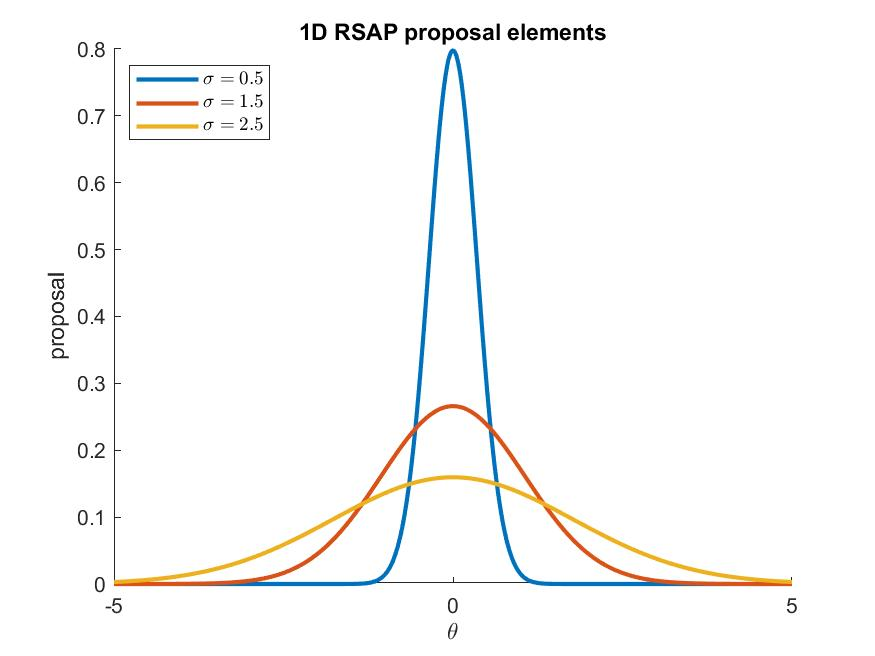
\includegraphics[scale = 0.2]{ProposalPlot_Separate}
	\endminipage\hfill %%%%%%%%%%%%%%%%%%%
	\minipage{0.5\textwidth}
		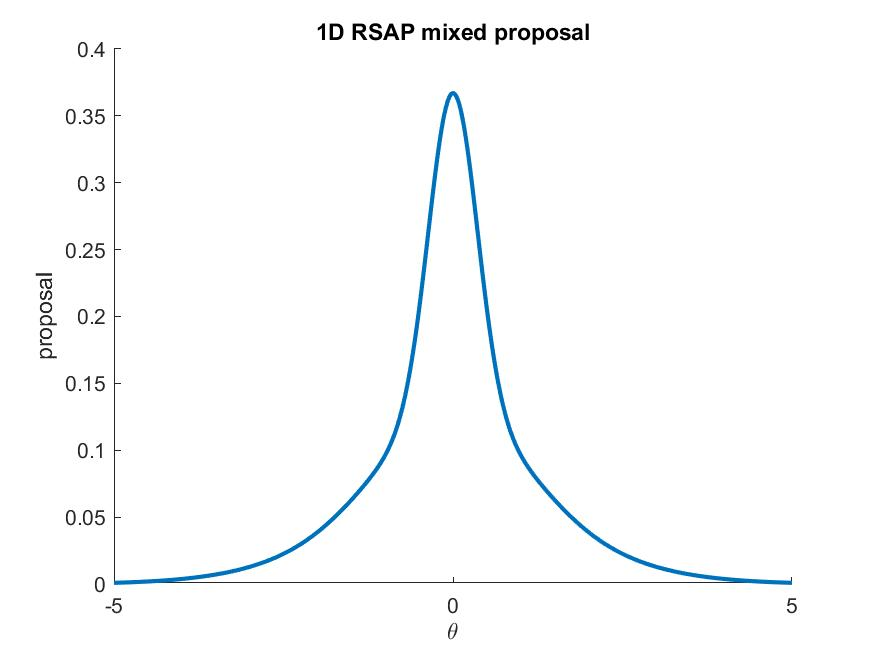
\includegraphics[scale = 0.2]{ProposalPlot_Mixed}
	\endminipage\hfill %%%%%%%%%%%%%%%%%%%
	\caption{RSAP proposal (Equation (\ref{Prop1D})) with $\sigma_t = 0.5, \sigma_f = 1.5, \sigma_w = 2.5, p_t = p_w = p_f = 1/3$.}
\end{figure}
Every parameter uses separately adapting wide and thin proposal widths---allowing for independent adaptation of each---as well as its own fixed width (since the different parameters likely have different units and/or scales).

The values of $\sigma_{t}^n, \sigma_{w}^n$ adapt based on the number of recent consecutive rejections the chain has encountered, with their default values set to $\sigma_{f}$. If the candidate produced by the method is rejected, we choose from the three kernels based on the defined mixing probabilities (which we will discuss in detail below). If the fixed kernel is chosen, then no adaptation is performed. However, if either the thin or wide kernels are used, then we increment one of the counters $k_{t}^n$, $k_{w}^n$ and compute the appropriate scale factor
\begin{equation}
	\begin{split}
		A_{t}(k_{t}^n) & = 1 - (1- \hat A_{t})(1-\textrm{exp}(-r_{t} k_{t}^n))\\
		A_{w}(k_{w}^n) & = 1 - (1- \hat A_{w})(1-\textrm{exp}(-r_{w} k_{w}^n))
	\end{split}
	\label{scaling}
\end{equation}
where $r_{w}>0$, $r_{t}>0$, $\hat A_{w}>1$, and $1>\hat A_{t}>0$. (These functions were chosen since their initial value is 1, their asymptotic limit is their respective $\hat A$ value, and their rate of convergence can be easily controlled via the $r$ constants.) We then set either $\sigma_{t}^n = A_{t}(k_{t}^n) \sigma_{f}$ or $\sigma_{w}^n = A_{w}(k_{w}^n) \sigma_{f}$ (depending on which was chosen) and perform a Metropolis step using this proposal width (again remembering that process is done independently for all parameters). On the other hand, whenever a candidate is accepted, the counters are reset to zero so that $\sigma_{t}^n = \sigma_{w}^n = \sigma_{f}$ (for all parameters).

Now, concerning how we choose between the three options, we have the time-dependent mixing probabilities $p_t^n, p_f^n, p_w^n$.
% that either the thin, fixed, or wide proposal (respectively) will be used.
The following formulae govern the specific behavior of these probabilities.
\begin{equation}
	\begin{split}
		p_f^n & = \left\{
						\begin{array}{ll}
							1/3 & \quad 0 \leq n < n_1 \\
							(2 - \textrm{cos}( \pi (n - n_1)/n_2))/3 & \quad n_1 \leq n < n_1 + n_2 \\
							1 & \quad n_1 + n_2 \leq n < N_{step}
						\end{array}
					\right.
		\\
		p_t^n = p_w^n & = (1 - p_f^n)/2
	\end{split}
	\label{mixing}
\end{equation}
The interval widths $n_1, n_2$ define three distinct regions for these functions. In the first region---which lasts $n_1$ steps---they describe a uniform distribution. In practice, $n_1$ should be set fairly large w.r.t. the total number of time steps $N_{step}$ so that RSAP has plenty of steps to utilize its adaptive features. The second region is a transition region---which lasts for $n_2$ steps---where proposal fixing begins to dominate the adaptation. The use of the cosine function here is somewhat arbitrary since any other function that is monotonically increasing on the interval $[n_1, n_1+n_2]$ would produce similar results. From the definitions of $p_t^n, p_w^n$, there is an equal probability at each step that either thinning or widening will be chosen. There is no firm guideline for setting the second interval except $n_1 + n_2 \le N_{step}$. With the last region, we forced eventual convergence to $p_f^n \rightarrow 1$, which---as we shall see---implies the ergodicity of RSAP (see Section 2.3).
\begin{figure}[!htb]
	\centering
	\minipage{0.5\textwidth}
		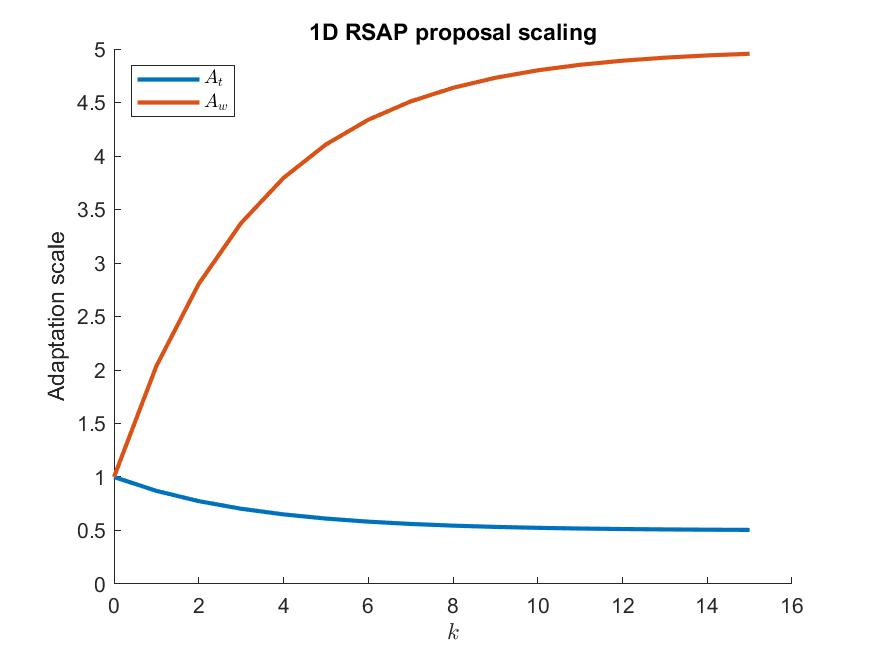
\includegraphics[scale = 0.22]{ProposalPlot_Scaling}
	\endminipage\hfill %%%%%%%%%%%%%%%%%%%
	\minipage{0.5\textwidth}
		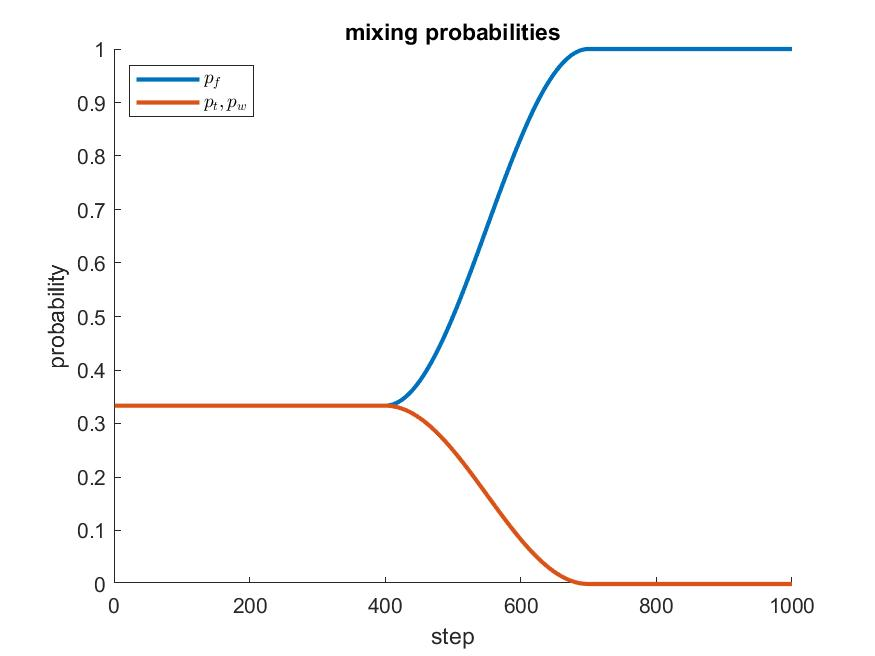
\includegraphics[scale = 0.22]{MixingProbabilities}
	\endminipage\hfill %%%%%%%%%%%%%%%%%%%
	\caption{Left: RSAP proposal-scaling functions \textnormal{(Equation (\ref{scaling}))} vs. adaptation degree $k$ with $r_t , r_w = 0.3, A_t = 0.5, A_w = 5$. Right: RSAP proposal-mixing probabilities \textnormal{(Equation (\ref{mixing}))} vs. time step with $n_1 = 400, n_2 = 300$.}
\end{figure}

To derive the full $M$-parameter proposal (which we do in Section 2.3 with the help of a great deal of added notation), one has to consider all $3^M$ possibilities of selecting the $M$ parameters and their three different types of adaptation. It is helpful to do a two-parameter example. Each parameter will have its own set of proposal widths $\sigma_{t,m}, \sigma_{f,m}, \sigma_{w,m}$ ($m=1,2$). Upon adaptation, both parameters must choose which form of adaptation to apply, meaning there are $3^2$ possibilities for adaptation. Therefore, for the sake of notation, defining $N(\theta^n, \sigma_1^2, \sigma_2^2)$ as a bivariate Gaussian distribution with diagonal covariance matrix given by the diagonal entries $(\sigma_1^2, \sigma_2^2)$, we can write the two-parameter proposal as (the superscript $n$'s for $\sigma$'s omitted for space reasons)
\begin{equation*}
	\begin{split}
		q^n(\theta'|\theta^n) = & \hspace{3pt} \sum_{i \in \{t,f,w\}} \sum_{j \in \{t,f,w\}} p_i^n p_j^n N(\theta^n,  \sigma_{i,1}^2, \sigma_{j,2}^2)
		\\
		= & \hspace{3pt} (p_t^n)^2 N(\theta^n, \sigma_{t,1}^2, \sigma_{t,2}^2) + p_t^n p_f^n N(\theta^n,  \sigma_{t,1}^2, \sigma_{f,2}^2) + p_t^n p_w^n N(\theta^n,  \sigma_{t,1}^2, \sigma_{w,2}^2) \hspace{3pt} +
		\\
		& \hspace{3pt} p_f^n p_t^n N(\theta^n,  \sigma_{f,1}^2, \sigma_{t,2}^2) + (p_f^n)^2 N(\theta^n, \sigma_{f,1}^2, \sigma_{f,2}^2) + p_f^n p_w^n N(\theta^n,  \sigma_{f,1}^2, \sigma_{w,2}^2) \hspace{3pt} +
		\\
		& \hspace{3pt} p_w^n p_t^n N(\theta^n, \sigma_{w,1}^2, \sigma_{t,2}^2) + p_w^n p_f^n N(\theta^n,  \sigma_{w,1}^2, \sigma_{f,2}^2) + (p_w^n)^2 N(\theta^n, \sigma_{w,1}^2, \sigma_{w,2}^2)
	\end{split}
\end{equation*}

% mention the communication theory thing Hugh said, look up paper

% (being diagonal, it merely equalizes the proposal width for the different parameters since they might be different units and, thus, have different scales)


Algorithm 2.1 provides a pseudocode representation of the method.
\begin{algorithm}[h]
\algsetup{
	indent=12pt,
	linenosize=\small,
	linenodelimiter=.
}
\begin{algorithmic}[1]
	\STATE Initialize $\theta^0$ %, $\hat \Sigma$, $k_{w}^m = 0$, $k_{t}^m = 0$ for all $m=1, ..., M$ - these conditions are redundant with the step after the second for loop
	
	\FOR{ $n = 1$ \TO $N_{step}$}  % the step number of the system
		\IF{ $n = 1$ \OR $\theta'^{,n-1}$ was accepted}
			\STATE Set $\Sigma = \hat \Sigma$, $k_{w}^{n,m} = 0$, $k_{t}^{n,m} = 0$ for all $m$
		\ELSE
			\FOR{ $m = 1$ \TO $M$}  %loop over the dimensions
				\STATE Choose from \{wide, thin, fixed\} with probabilities \{$p_w^n, p_t^n, p_f^n$\}
%				\IF[increase]{0}
				\IF{wide}
					\STATE $k_{w}^{n,m} = k_{w}^{n-1,m} + 1$
					\STATE $A_{w}^m = 1 - (1-\hat A_{w})(1-\textrm{exp}(-r_{w} k_{w}^{n,m}))$
					\STATE $\Sigma_{m,m} = A_{w}^m \hat \Sigma_{m,m}$
%				\ELSIF[decrease]{1}
				\ELSIF{thin}
					\STATE $k_{t}^{n,m} = k_{t}^{n-1,m} + 1$
					\STATE $A_{t}^m = 1 - (1-\hat A_{t})(1-\textrm{exp}(-r_{t} k_{t}^{n,m}))$
					\STATE $\Sigma_{m,m} = A_{thin}^m \hat \Sigma_{m,m}$
%				\ELSE[initial]
				\ELSE
					\STATE $\Sigma_{m,m} = \hat \Sigma_{m,m}$
				\ENDIF
			\ENDFOR
		\ENDIF
		\STATE Generate $\theta'^{,n} \sim N(\theta^{n-1},\Sigma)$
		\STATE Compute $\alpha(\theta'^{,n}|\theta^{n-1}) =\textrm{min}\Bigg(1, \dfrac{\ell(y|\theta'^{,n})p(\theta'^{,n})} {\ell(y|\theta^{n-1})p(\theta^{n-1})}\Bigg)$
		\STATE Set $\theta^n = \theta'^{,n}$ with probability $\alpha$, else $\theta^n = \theta^{n-1}$
	\ENDFOR
\end{algorithmic}
\caption{Rejection-scaled adaptive proposal (RSAP)}
\end{algorithm}
We use a uniform prior over the given domain and a diagonal covariance matrix $\hat \Sigma$ for our fixed Gaussian. We define $N_{step}$ as the number of time steps and $M$ as the number of parameters. We also define separate counters $k_{w}^m$, $k_{t}^m$ for every parameter $m = 1, ..., M$. As can clearly be seen, lines 3-20 are the additional adaptive functionality while lines 21-23 are from the standard Metropolis method.


\subsection{Ergodicty of RSAP}
We will now demonstrate the ergodicity of RSAP by proving that conditions $a$ and $b$ of Theorem 5 from Roberts and Rosenthal \cite{RRAdaptErgo} hold for our method. Theorem 5 states
\begin{theorem}
	[Theorem 5 \cite{RRAdaptErgo}] Consider an adaptive MCMC algorithm, on a state space $\mathcal{X}$, with adaptation index $\mathcal{Y}$, so $\pi( \cdot )$ is stationary for each kernel $P_y$ for $y \in \mathcal{Y}$. Assume that:
	\begin{tight_enum}
		\item \textnormal{(Simultaneous Uniform Ergodicity)} For all $\epsilon > 0$, there $N = N(\epsilon) \in \mathbb{N}$ such that $||P^N_y(x, \cdot) - \pi(\cdot)|| \le \epsilon$ for all $x \in \mathcal{X}$ and $y \in \mathcal{Y}$.
		\item \textnormal{(Diminishing Adaptation)} The limit $\lim_{n \rightarrow \infty} D_n = 0$ in probability, where $D_n = \sup_{x \in \mathcal{X}} ||P_{\Gamma_{n+1}}(x, \cdot) - P_{\Gamma_{n+1}}(x, \cdot)||$ is a $\mathcal{G}_{n+1}$-measurable random variable \textnormal{(}depending on the random values $\Gamma_n$ and $\Gamma_{n+1}$\textnormal{)}.
	\end{tight_enum}
	\hspace{15pt} Then the adaptive algorithm is ergodic.
	\label{ErgoThm}
\end{theorem}
More plainly, the theorem states that an adaptive method is ergodic if it is ($a$) \textit{simultaneously uniformly ergodic} and has ($b$) \textit{diminishing adaptation}. Condition $a$ means that all proposals which could be used in the adaptive method are themselves ergodic if used as proposals for standard Metropolis. Condition $b$ means that the ``amount of adaptation" eventually vanishes, i.e., that the sequence of proposals converges (see \cite{RRAdaptErgo} for more rigorous definitions as well as a proof of Theorem 5). Condition $a$ clearly holds in the case of RSAP since the proposals are all Gaussians, which are ergodic. Therefore, the remainder of this section will be devoted to proving ($b$).

\subsubsection{Proving diminishing adaptation}

Suppose there are $M$ parameters which RSAP must estimate and that $\hat \Sigma$ is a fixed diagonal covariance matrix for these parameters. First, define the following as the \textit{elemental proposals}
\begin{equation*}
	E \Big( (j_1,i_1), \cdots, (j_M, i_M) \Big) = 	N(\theta^n, \Sigma)
\end{equation*}
where
\begin{equation*}
	\Sigma_{m,m} = 
	\left\{
		\begin{array}{ll}
			\hat \Sigma_{m,m} \cdot A_{t}(i_m) & \quad j_m = 1 \\
			\hat \Sigma_{m,m} & \quad j_m = 2 \\
			\hat \Sigma_{m,m} \cdot A_{w}(i_m) & \quad j_m = 3
		\end{array}
	\right.
\end{equation*}
with their respective \textit{acceptance probabilities} $a^n_{(j_1,i_1), \cdots, (j_M,i_M)} = \alpha(\theta'|\theta^n)$ where $\theta'$ was drawn from the elemental proposal described by the subscripts and $m = 1, \cdots, M$. We let $n$ be the time step, the $i_m$'s be the adaptation degrees, and the $j_m$'s be switches that determine to which mode of adaptation the $i_m$'s are applied (1 = thin, 2 = fixed, 3 = wide). Note that $n$ and $i_m$ are non-negative integers such that $n \ge i_m$ since, in practice, the degree of adaptation cannot exceed the number of time steps which have occured. For the sake of notational simplicity, we will also define the \textit{rejection probabilities} $r^n_{(j_1,i_1), \cdots, (j_M,i_M)} = 1- a^n_{(j_1,i_1), \cdots, (j_M,i_M)}$.

Next, define the following linear combinations as the \textit{adaptive proposals}
\begin{equation}
	q^n_{i^1_1, i^2_1, i^3_1, \cdots, i^1_M, i^2_M, i^3_M} = \sum^{3}_{j_1=1} p_{j_1}^n \cdots \sum^{3}_{j_M=1} p_{j_M}^n E \Big( (j_1,i^{j_1}_1), \cdots, (j_M, i^{j_M}_M) \Big)
	\label{adaPro}
\end{equation}
with their associated \textit{acceptance probabilities}
\begin{equation*}
	b^n_{i^1_1, i^2_1, i^3_1, \cdots, i^1_M, i^2_M, i^3_M} = \sum^{3}_{j_1=1} p_{j_1}^n \cdots \sum^{3}_{j_M=1} p_{j_M}^n a^n_{(j_1,i^{j_1}_1), \cdots, (j_M, i^{j_M}_M)}
\end{equation*}
%for all $n = \sum_{j = 1}^{3} i^j_m$.
This is the $M$-parameter generalization of the one- and two-parameter proposals from Section 2.2 with the subscripts $t,f,w$ replaced with $1,2,3$, respectively. Let's examine Equation (\ref{adaPro}) more closely before continuing on. Regarding the indices, the integers $i^1_m$ are the degrees of proposal-\textit{thinning} adaptation while the integers $i^3_m$ are the degrees of proposal-\textit{widening} adaptation. The integers $i^2_m$ can be thought of as the degrees of proposal-\textit{fixing} adaptation (clearly a meaningless notion). They are merely auxiliary indices which help to establish conservation of adaptation degrees. Regarding the sums, there is one per parameter and their indices cover the three adaptation options so that the probability of choosing the elemental proposal $E((j_1,i^{j_1}_1), \cdots, (j_M, i^{j_M}_M))$ is $p_{j_1}^n \cdots p_{j_M}^n$.

\begin{comment}
A helpful (though not exactly correct) way to think about the generalization from $\hat q$ to $q'$ is to think of $q'$ as an $M$-fold direct product of $\hat q$ with itself. Abusing notation momentarily, define $E((s_1,k_1)) \times E((s_2, k_2)) = E((s_1,k_1), (s_2, k_2))$. Then, $q'$ can be written
\begin{equation}
	q'_{i^1_1, i^2_1, i^3_1, \cdots, i^1_M, i^2_M, i^3_M} =  \prod_{m=1}^{M} \dfrac{1}{3} \bigg( E((1,i^{1}_m)) + E((2,i^{2}_m)) + E((3,i^{3}_m)) \bigg)
\end{equation}
(This equation is written for purely instructive purposes, and is not utilized in any way in the proof or the algorithm itself.)
\end{comment}

Lastly, define $Q^n$ as the \textit{full proposal} at time-step $n$. Since acceptance and rejection are random phenomena, we cannot know ahead of time which specific elemental or adaptive proposal will be used at time step $n$. Thus, the full proposal will be a linear combination of the adaptive proposals whose total adaptation degrees are less than or equal to $n$ (since there could only have been up to $n$ rejections and, therefore, $n$ adaptations) with functions of their respective acceptance probabilities. In what follows, we will show how to build $Q^n$ from the objects we defined above.

Let us now examine the structure of the full proposal and how it evolves throughout a run, temporarily restricting ourselves to one dimension for simplicity. Below, Figure 1 provides a graphical representation of the flow of proposals during a run (with the time step superscripts ommitted).
\begin{figure}[!h]
	\centering
	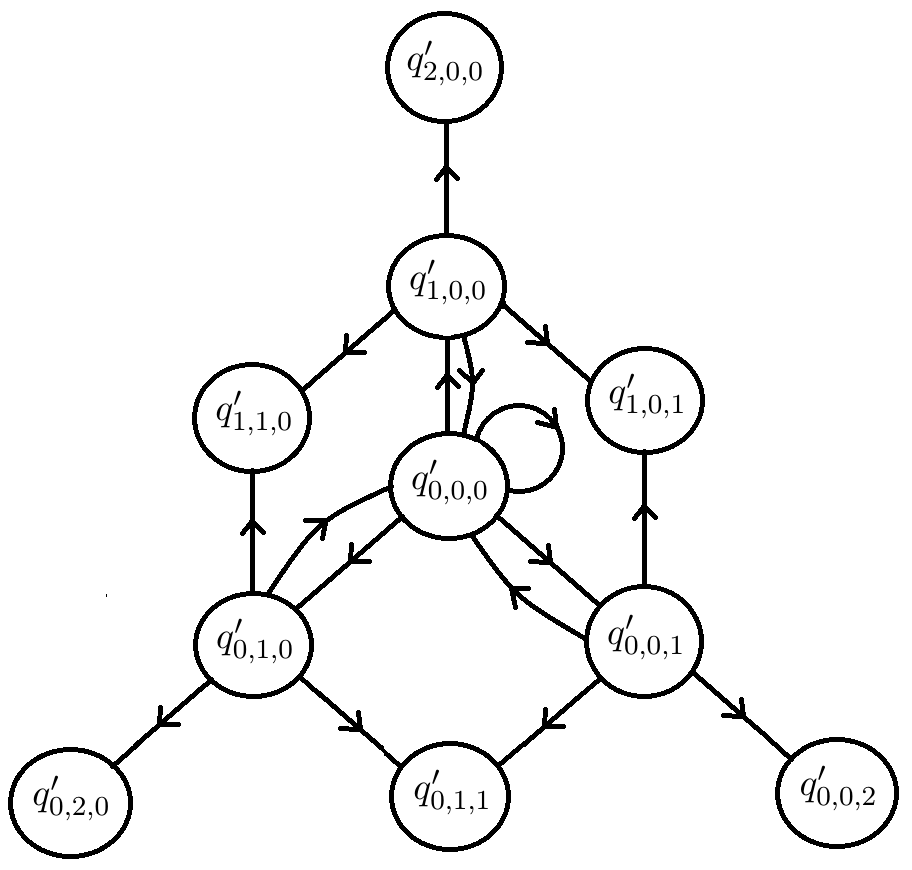
\includegraphics[scale = 0.3]{RSAP_True_02}
%	\vspace{-40pt}
	\caption{A graphical depiction of RSAP and the possible transitions that can take place. At any node (\textit{adaptive} proposal) in the graph, four transitions can occur: increasing one of the three indices (rejection) or returning to the initial state (acceptance). Note that we have omitted the time step superscript since to properly represent the method graphically would require another dimension to represent time. We instead identify all the proposals with the same adaptation degrees and simply use primes to denote the fact that they represent numerous other proposals with equivalent adaptation degrees but larger time step superscripts.}%a transition must take place between time steps (i.e. increments the superscript), thus making it unclear which step value any of the nodes on the graph should be given, particularly for the center, un-adapted node/proposal.}
%. SHOULD THIS GRAPH HAVE ANY RETURN LOOPS?   IT MAY BE CONFUSING TO HAVE STATES FROM Q001 TO Q000 BUT NOT FROM THE OTHERS.	
\end{figure}
One can think of method runs as paths through this graph. The first proposal is always $q^0_{0,0,0}$ since no adaptation has yet taken place. Consequently, the first full proposal $Q^0$ is also $q^0_{0,0,0}$. As illustrated by the graph, there are four possible transitions from any given proposal. If acceptance occurs, the adaptation returns to $q^0_{0,0,0}$ (the fixed proposal with no adaptation). Alternatively, if rejection occurs, we will increment the adaptive degree indices corresponding to the elemental proposal which was used. For example---beginning with $q^0_{0,0,0}$---suppose that rejection occurs and thinning was the chosen mode of adaptation. Then, we increment the thin proposal index so that the adaptive proposal used in the next time step will be $q^1_{1,0,0}$. We can represent this mathematically with linear combinations of the adaptive proposals. Equations (\ref{exQ}) below show the full proposals through $q^2$.
\begin{equation}
	\begin{split}
		Q^0 = & \hspace{3pt} q_{0,0,0}^0 
		\\[5pt]
		Q^1 = & \hspace{3pt} b^0_{0,0,0} q_{0,0,0}^1 + r^0_{(1,0)} p^0_1 q_{1,0,0}^1 + r^0_{(2,0)} p^0_2 q_{0,1,0}^1 + r^0_{(3,0)} p^0_3 q_{0,0,1}^1
		\\[5pt]
		Q^2 = & \hspace{3pt} \Big( b^1_{0,0,0} b^0_{0,0,0} + b^1_{1,0,0} r^0_{(1,0)} p^0_1 + b^1_{0,1,0} r^0_{(2,0)} p^0_2 + b^1_{0,0,1} r^0_{(3,0)} p^0_3 \Big) q_{0,0,0}^2 + 
		\\
		& \hspace{3pt} r^1_{(1,0)} p^1_1 b^0_{0,0,0} q_{1,0,0}^2 + r^1_{(2,0)} p^1_2 b^0_{0,0,0} q_{0,1,0}^2 + r^1_{(3,0)} p^1_3 b^0_{0,0,0} q_{0,0,1}^2 +
		\\
		& \hspace{3pt} r^1_{(1,1)} p^1_1 r^0_{(1,0)} p^0_1 q_{2,0,0}^2 + r^1_{(2,1)} p^1_2 r^0_{(1,0)} p^0_1 q_{1,1,0}^2 + r^1_{(3,1)} p^1_3 r^0_{(1,0)} p^0_1 q_{1,0,1}^2 +
		\\
		& \hspace{3pt} r^1_{(1,1)} p^1_1 r^0_{(2,0)} p^0_2 q_{1,1,0}^2 + r^1_{(2,1)} p^1_2 r^0_{(2,0)} p^0_2 q_{0,2,0}^2 + r^1_{(3,1)} p^1_3 r^0_{(2,0)} p^0_2 q_{0,1,1}^2 +
		\\
		& \hspace{3pt} r^1_{(1,1)} p^1_1 r^0_{(3,0)} p^0_3 q_{1,0,1}^2 + r^1_{(2,1)} p^1_2 r^0_{(3,0)} p^0_3 q_{0,1,1}^2 + r^1_{(3,1)} p^1_3 r^0_{(3,0)} p^0_3 q_{0,0,2}^2
	\end{split}
	\label{exQ}
\end{equation}
As can be seen (and was mentioned earlier), $Q^n$ contains all adaptive proposals of total degree up to $n$, i.e., $i_1^1+i_1^2+i_1^3 \le n$ (for $M$ parameters, this inequality holds for all parameters simultaneously). Therefore, we can express $Q^n$ neatly as
\begin{equation*}
	Q^n = \sum^n_{\ell=0} \Bigg(\sum_{i_1^1+i_1^2+i_1^3=\ell} c^n_{i_1^1,i_1^2,i_1^3} q_{i_1^1,i_1^2,i_1^3}^n \Bigg)
\end{equation*}
where
\begin{align*}
	\sum^n_{\ell=0} \Bigg(\sum_{i_1^1+i_1^2+i_1^3=\ell} c^n_{i_1^1,i_1^2,i_1^3} \Bigg) = 1
\end{align*}
defines our normalization (since some proposal must always be chosen) and the inner sums are taken over all possible values of the three indices such that their sum is less than or equal to $\ell$. The value $c^n_{i_1^1,i_1^2,i_1^3}$ can be interpreted as the probability that that the adaptive proposal defined by the subscripts will be used at step $n$.

Now, returning to $M$ parameters, let us generalize the above formulae. The full proposal is written
\begin{equation*}
	Q^n = \sum^n_{\ell=0} \Bigg(\sum_{i^1_m+i^2_m+i^3_m=\ell} c^n_{i^1_1, i^2_1, i^3_1, \cdots, i^1_M, i^2_M, i^3_M} q_{i^1_1, i^2_1, i^3_1, \cdots, i^1_M, i^2_M, i^3_M}^n \Bigg)
\end{equation*}
with analogous normalization condition
\begin{align*}
	\sum^n_{\ell=0} \Bigg(\sum_{i^1_m+i^2_m+i^3_m=\ell} c^n_{i^1_1, i^2_1, i^3_1, \cdots, i^1_M, i^2_M, i^3_M} \Bigg) = 1
\end{align*}
where $m = 1, \cdots, M$. We can construct several recurrence relations which describe how the values of the coefficients $c^n$ change over time. We get one relation which governs the evolution of the coefficient corresponding to the proposal which has zero total adaptation degree and another which governs the rest.
\begin{equation}
	\begin{split}
		c^{n+1}_{0,0,0, \cdots, 0,0,0} = & \hspace{3pt} \sum^n_{\ell=0} \Bigg( \sum_{i^1_m+i^2_m+i^3_m=\ell} \Big( b^n_{i^1_1, i^2_1, i^3_1, \cdots, i^1_M, i^2_M, i^3_M} \Big) \Big( c^n_{i^1_1, i^2_1, i^3_1, \cdots, i^1_M, i^2_M, i^3_M} \Big) \Bigg)
		\\
		c^{n+1}_{i^1_1, i^2_1, i^3_1, \cdots, i^1_M, i^2_M, i^3_M} = & \hspace{3pt} \sum_{j_1 \mid i^{j_1}_1 \ge 1} \cdots \sum_{j_M \mid i^{j_M}_M \ge 1} \Big( r^n_{(j_1,i^{j_1}_1), \cdots, (j_M,i^{j_M}_M)} \Big) \Big( p^n_{j_1} \cdots p^n_{j_M} \Big) \times
		\\
		& \hspace{3pt} \Big( c^{n}_{i^1_1, \cdots, i^{j_1}_1-1, \cdots, i^3_1, \cdots, i^1_M, \cdots, i^{j_M}_M-1, \cdots, i^3_M} \Big)
	\end{split}
	\label{recur}
\end{equation}
The first relation is fairly basic, as it simply was derived from the fact that the adaptation-free proposal will be used at any step which immediately follows an acceptance. Consequently, it finds the total, weighted acceptance probability given all possible proposals which could be used at that step. This is equal to the probability that the adaptation-free proposal will be chosen at the following step.

The second relation is more complicated. The summations are over all values $j_m$ such that $i_m^{j_m} \ge 1$ for $m = 1, \cdots, M$. Conceptually, the relation finds the total, weighted rejection probability from all proposals which could possibly precede the proposal under consideration. More specifically, it does this by summing the weighted rejection probabilities over all valid configurations
% permutations (original, wrong)
% instances
% configurations
% sets
% groups
of subtracting one from the three types adaptation degrees for all $M$ parameters (of which there are no more than $3^M$ possible configurations). A configuration is considered valid when subtracting one does not give a negative adaptation degree (thus the $i^{j_m}_m \ge 1$ under the sums).

% is it confusing which time step is being referred to as current/previous?

Now, to prove diminishing adaptation, we will show that the values of $c^{n}_{i^1_1, i^2_1, i^3_1, \cdots, i^1_M, i^2_M, i^3_M}$ vanish as $n \rightarrow \infty$ for any proposals that have at least one degree of either thinning or widening adaptation in at least one parameter. We will use induction on the thinning and widening adaptation degrees to prove this.

Let us first prove the base case, where we consider a proposal such that each parameter has only one adaptation degree assigned and there exists at least one parameter such that its mode of adaptation is either thinning or widening. Without loss of generality, we will say that this is the first parameter and that thinning was chosen (the widening case is identical).
%Letting $c^{n}_{1, 0, 0, \cdots, i^1_M, i^2_M, i^3_M}$ be the coefficient of this proposal, this implies that either $i^1_m=1$ or $i_m^3=1$ for every $m = 2, \cdots, M$.
Let $c^{n}_{1, 0, 0, \cdots, i^1_M, i^2_M, i^3_M}$ be the coefficient of this proposal. Then, using the recurrence relation, we get
\begin{equation*}
	c^{n+1}_{1, 0, 0, \cdots, i^1_M, i^2_M, i^3_M} = \Big( r^n_{(1,0), \cdots, (j_M,i^{j_M}_M)} \Big) \Big( p^n_{1} \cdots p^n_{j_M} \Big) \Big( c^{n}_{0,0,0, \cdots, 0,0,0} \Big)
\end{equation*}
Now, all the terms in this equation are bounded between 0 and 1 and $p_1^n \rightarrow 0$ as $n \rightarrow \infty$. Therefore, $c^{n+1}_{1, 0, 0, \cdots, i^1_M, i^2_M, i^3_M} \rightarrow 0$, as well, and we have that all coefficients with at least one parameter having a single adaptive degree assigned to either thinning or widening vanish.

We will now prove the induction step, which states that if any coefficient with at least one parameter having at least one thinning or widening adaptive degree vanishes, then the coefficients for all proposals that it precedes by one adaptation degree of any kind (in the sense of the discussion of Equation (\ref{recur})) vanish as well. Consider $c^{n}_{i^1_1, i^2_1, i^3_1, \cdots, i^1_M, i^2_M, i^3_M}$, which has at least one parameter with at least one thinning or widening adaptive degree. Equation (\ref{recur}) applied to this coefficient contains the coefficients for all possible preceding states. Now, since there is at least one degree of thinning or widening adaptation in the coefficient under consideration, every term in the sum from Equation (\ref{recur}) can be classified in one of two ways: either 1) that adaptation degree was obtained from the immediately preceding step or 2) from an earlier step. If it is from the immediately preceding step, we can factor out the appropriate probability term as we did for the base case, causing that term to vanish. If it was from an earlier step, then the proposal associated with that term already has at least one parameter with at least one thinning or widening adaptive degree, and thus---according to the induction hypothesis---vanishes. Having shown that every term in the sum vanishes, we have shown that all proposal coefficients with at least one parameter with at least one thinning or widening adaptive degree also vanish. Thus, the only non-vanishing coefficients are those for purely fixing proposals, which are all identical to the adaptation-free proposal. Therefore, the full proposal $Q^n \rightarrow q^{n}_{0,0,0, \cdots, 0,0,0}$ as $n \rightarrow \infty$, thus proving part ($b$) of Theorem \ref{ErgoThm}, i.e., diminishing adaptation. Therefore, having proven both ($a$) and ($b$), we have also proven the ergodicity of RSAP.

It is readily apparent that we took advantage of the ergodicity of Metropolis in order to prove the ergodicity of RSAP. In fact, the convergence of the mixing probabilities to $p_f^n \rightarrow 1$ essentially forces the method into Metropolis over time. We suspect, however, that RSAP might be ergodic without this condition on the mixing probabilities. Proving this would require showing that Equation (\ref{recur}) implies that the $c^n$'s converge in distribution. They certainly do not directly converge in value since they depend on the acceptance/rejeciton probabilities which are highly volatile; however, an argument can likely be made that this implies their convergence in distribution. We will leave this for a future paper since the current version of RSAP is sufficient.


\section{Computational testing}
Having proven the %analytical integrity 
ergodicity of our method, we now move on to demonstrate its practical utility through the presentation of numerous computational results which cover multiple different aspects of the method's performance, including its flexibility, mixing efficiency, and convergence properties. We also present results from a new optimization-style test that we developed in which we find the cumulative probability distribution for convergence of the chain to the posterior's global maximum (or the minimum of the test function) versus a range of fixed proposal widths. This technique provides easy-to-interpret results which are numerically \textit{and} visually simple to compare. This test will be applied to RSAP, Metropolis, and Adaptive Metropolis from Section 1.3.


\subsection{Discussion of RSAP and modified AM parameter values used in testing}
When performing numerical experiments on our method, we used standard optimization test functions, each with a global minimum of $y = f(\theta^*) = 0$ (the bi-modal function has two adjacent minima). As such, the likelihood function can be expressed as
\begin{equation*}
	\begin{split}
		\ell(y|\theta) & \propto \textrm{exp}\bigg(-\dfrac{1}{2} \dfrac{(y-f(\theta))^2}{\Delta^2}\bigg)\\
					& \propto \textrm{exp}\bigg(-\dfrac{1}{2} \dfrac{f(\theta)^2}{\Delta^2}\bigg)\\
	\end{split}
\end{equation*}
The value of $\Delta$ is related to the scale of the error. It also affects the ease of acceptance, and thus the relative peakedness of the resulting sample-binned approximation of the posterior. Not knowing its proper value, we include it as a parameter for RSAP to estimate, though we set its proposal width quite low so that it does not change too rapidly, dramatically altering the acceptance rate.%(we further discuss this parameter and its effects on performance in Section 3.3).

There is also the matter of setting the adaptation parameters to their proper values. Clearly, the optimal values of these parameters are problem-dependent; so we attempted to find a set of reasonable values which improved the performance gain for as many test cases as possible. We thus arrived at scaling magnitudes of $\hat A_{t} = 0.1, \hat A_{w} = 10$, respectively. Being able to both increase and decrease the proposal width by an order of magnitude ensures that the true optimal width is likely contained within the interval $[\hat A_t \sigma_f, \hat A_w \sigma_f]$. Next, concerning the scaling rates, we found that their values were less significant than the magnitudes in determining performance gain. Their values were set to $r_{t}, r_{w} = 0.3$, since this puts the scaling to within approximately 5\% of its maximum effect within 10 rejection steps ($e^{-0.3 \cdot 10} \approx 0.049$). Smaller rate values would require more consecutive rejections to reach the same amount of scaling, thus wasting valuable time. Lastly, the interval widths $n_1, n_2$ are likely the most problem-dependent parameters since they determine how long RSAP is allowed to be adaptive. As discussed earlier, $n_1$ should be large w.r.t. $N_{step}$ while $n_2 \leq N_{step} - n_1$ has more freedom.

Concerning AM, we ran the method for $N_{burn}$ steps using the same fixed proposal widths as the other two methods. Once these steps have passed, we begin using the AM proposal, ignoring the first half of the initial burn-in steps in all of the subsequent covariance calculations. This is so that the covariance matrix calculations aren't as biased by the choice of initial state. Also, we set $\varepsilon = 0.001$ for all of the tests.

\subsection{Chain mixing}
% https://python-graph-gallery.com/111-custom-correlogram/
To begin the discussion of our results, we will provide trace plots of one-parameter chains created by RSAP for the test functions under consideration, as well as plots of the functions used and sample-binned approximations of the posterior distribution. We will start with the 1D Gaussian defined by
\begin{equation*}
	f(\theta) = a \Big( 1 - \textrm{exp}(-\dfrac{1}{2} \dfrac{\theta^2}{b^2}) \Big)
\end{equation*}
where $a = 1, b = 0.3, \theta \in [-1, 1]$. The initial state values were set to $\theta^0 = 0.8, \Delta^0 = 0.08$ and the fixed proposal widths were set to $\sigma_\theta = 0.1, \sigma_\Delta = 0.0008$. As discussed above, the parameters for RSAP were set to $\hat A_{t} = 0.1, \hat A_{w} = 10, r_{t} = 0.3, r_{w} = 0.3, n_1 = 2000, n_2 = 1000$.
\begin{figure}[!htb]
\minipage{0.33\textwidth}
	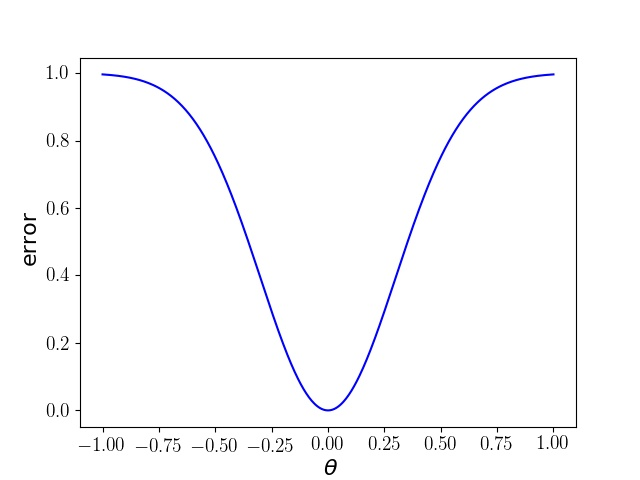
\includegraphics[width=\linewidth]{UQPlot_Gaussian_00_Function.jpg}
\endminipage\hfill
\minipage{0.33\textwidth}
	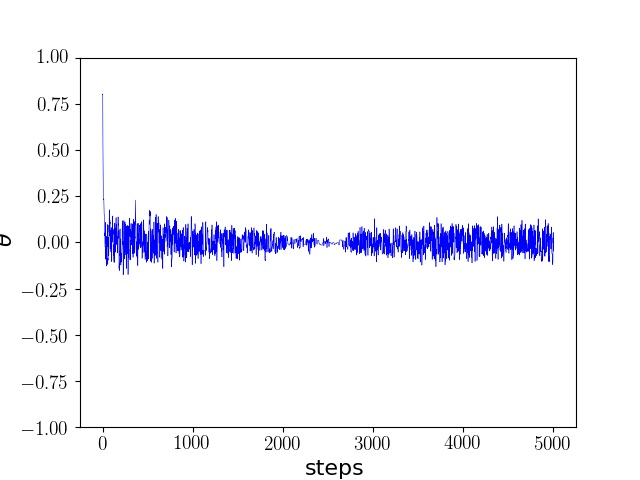
\includegraphics[width=\linewidth]{UQPlot_Gaussian_00_Trace.jpg}
\endminipage\hfill
\minipage{0.33\textwidth}%
	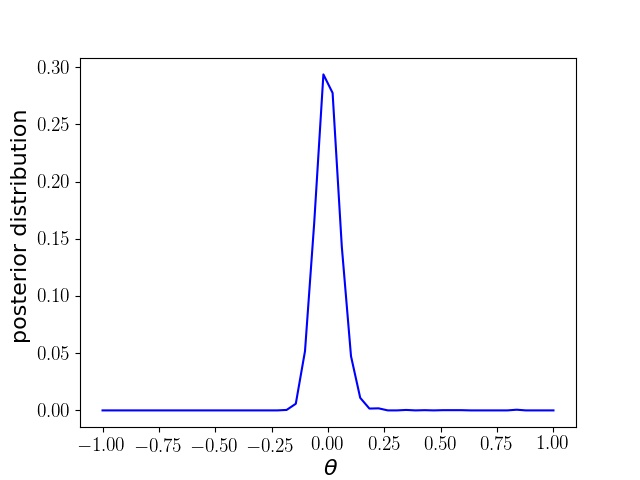
\includegraphics[width=\linewidth]{UQPlot_Gaussian_00_Posterior.jpg}
\endminipage
\caption{Plots of the Gaussian function (left), chain trace (center), and binned posterior estimate (right) resulting from a run with 5,000 steps. For the posterior plot on the right, we used 50 bins, giving a bin width of 0.04.}
\end{figure}
We use the Gaussian as a control example since it is such a simple function and does not require adaptation.

Next, we have an Ackley function in 1D defined by
\begin{equation*}
	f(\theta) = a \Big( 1 - \textrm{exp}(- 0.2 \sqrt{\theta^2/M}) \Big) + b \Big( e - \textrm{exp}(\textrm{cos}(2 \pi \theta)/M) \Big)
\end{equation*}
where $a = 20, b = 4, M = 1, \theta \in [-10, 10]$. The initial state values were set to $\theta_0 = 8, \Delta_0 = 3.5$ and the fixed proposal widths were set to $\sigma_\theta = 1.0, \sigma_\Delta = 0.01$. The RSAP parameters again were set to $\hat A_{t} = 0.1, \hat A_{w} = 10, r_{t} = 0.3, r_{w} = 0.3, n_1 = 2000, n_2 = 1000$.
\begin{figure}[!htb]
\minipage{0.33\textwidth}
	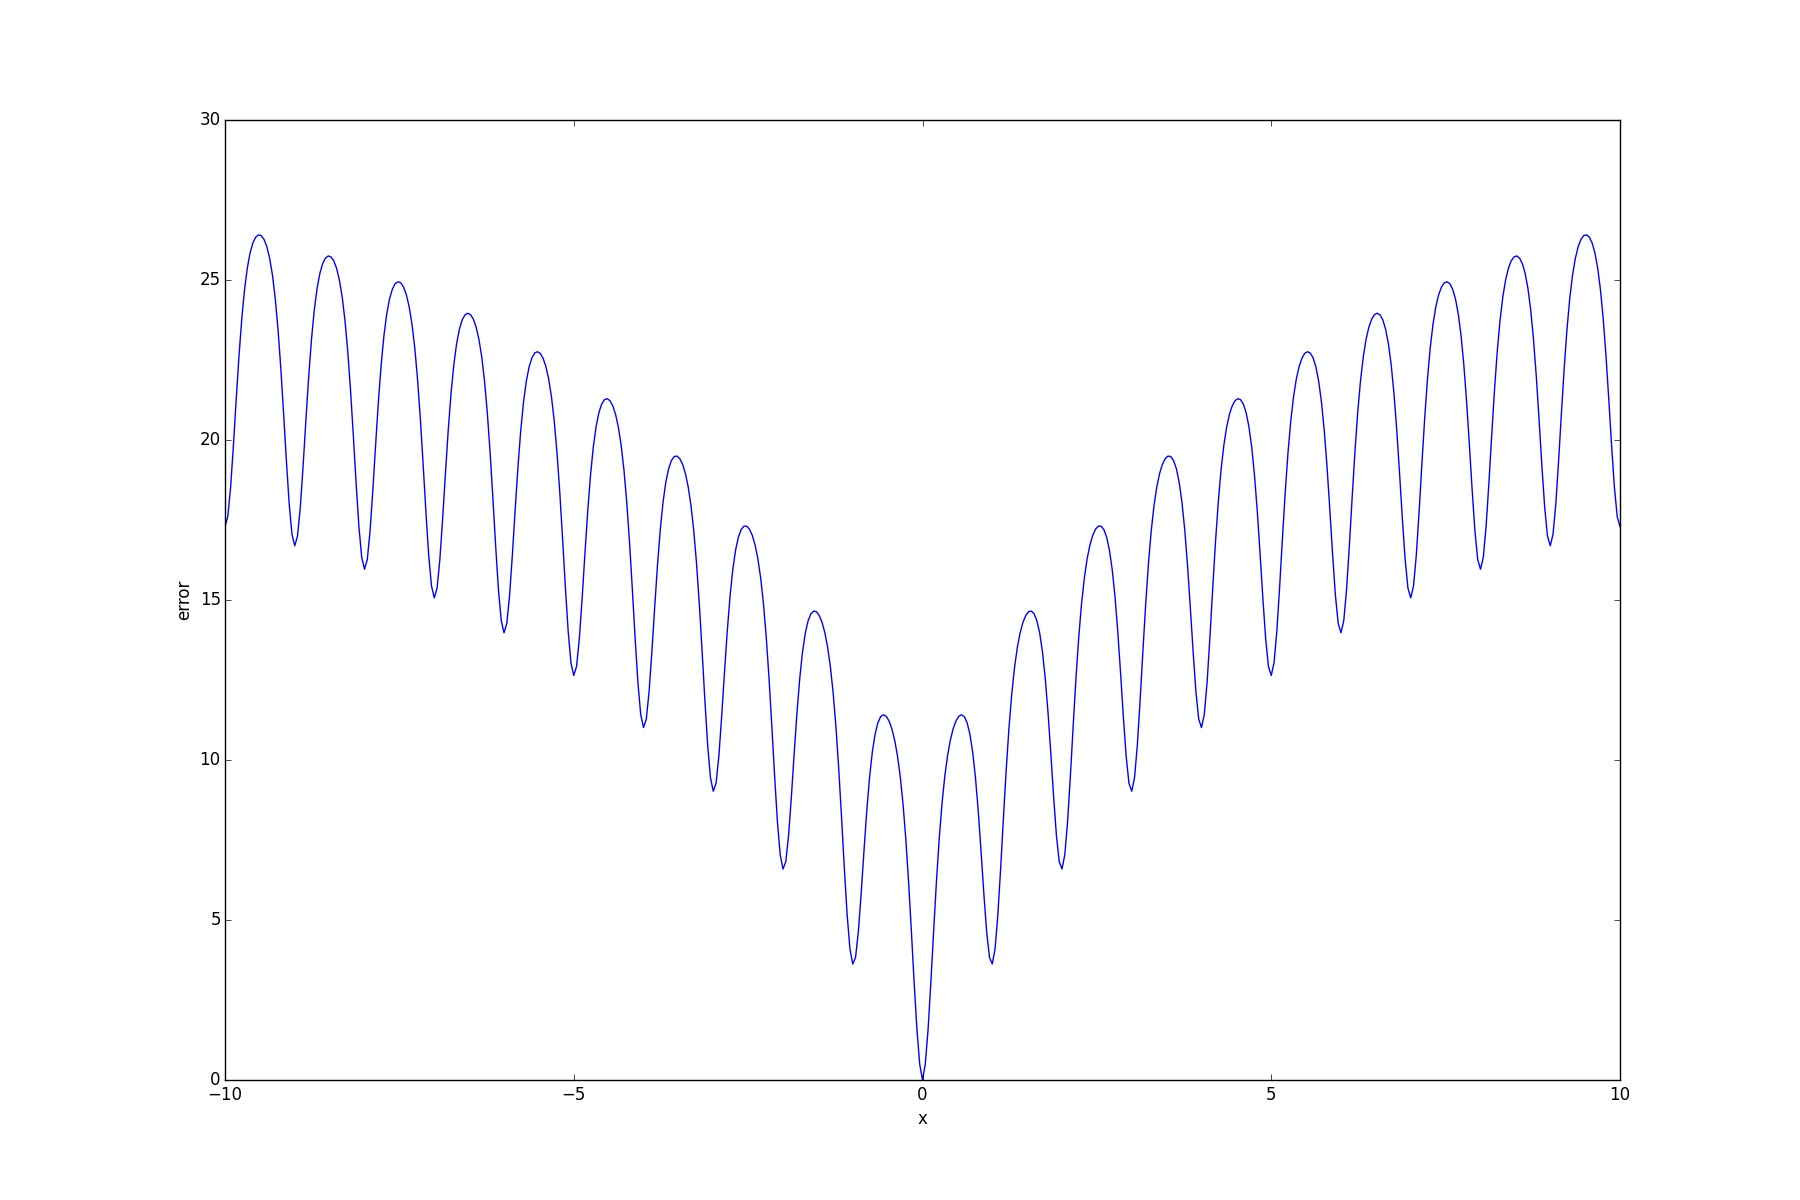
\includegraphics[width=\linewidth]{UQPlot_Ackley_00_Function.jpg}
\endminipage\hfill
\minipage{0.33\textwidth}
	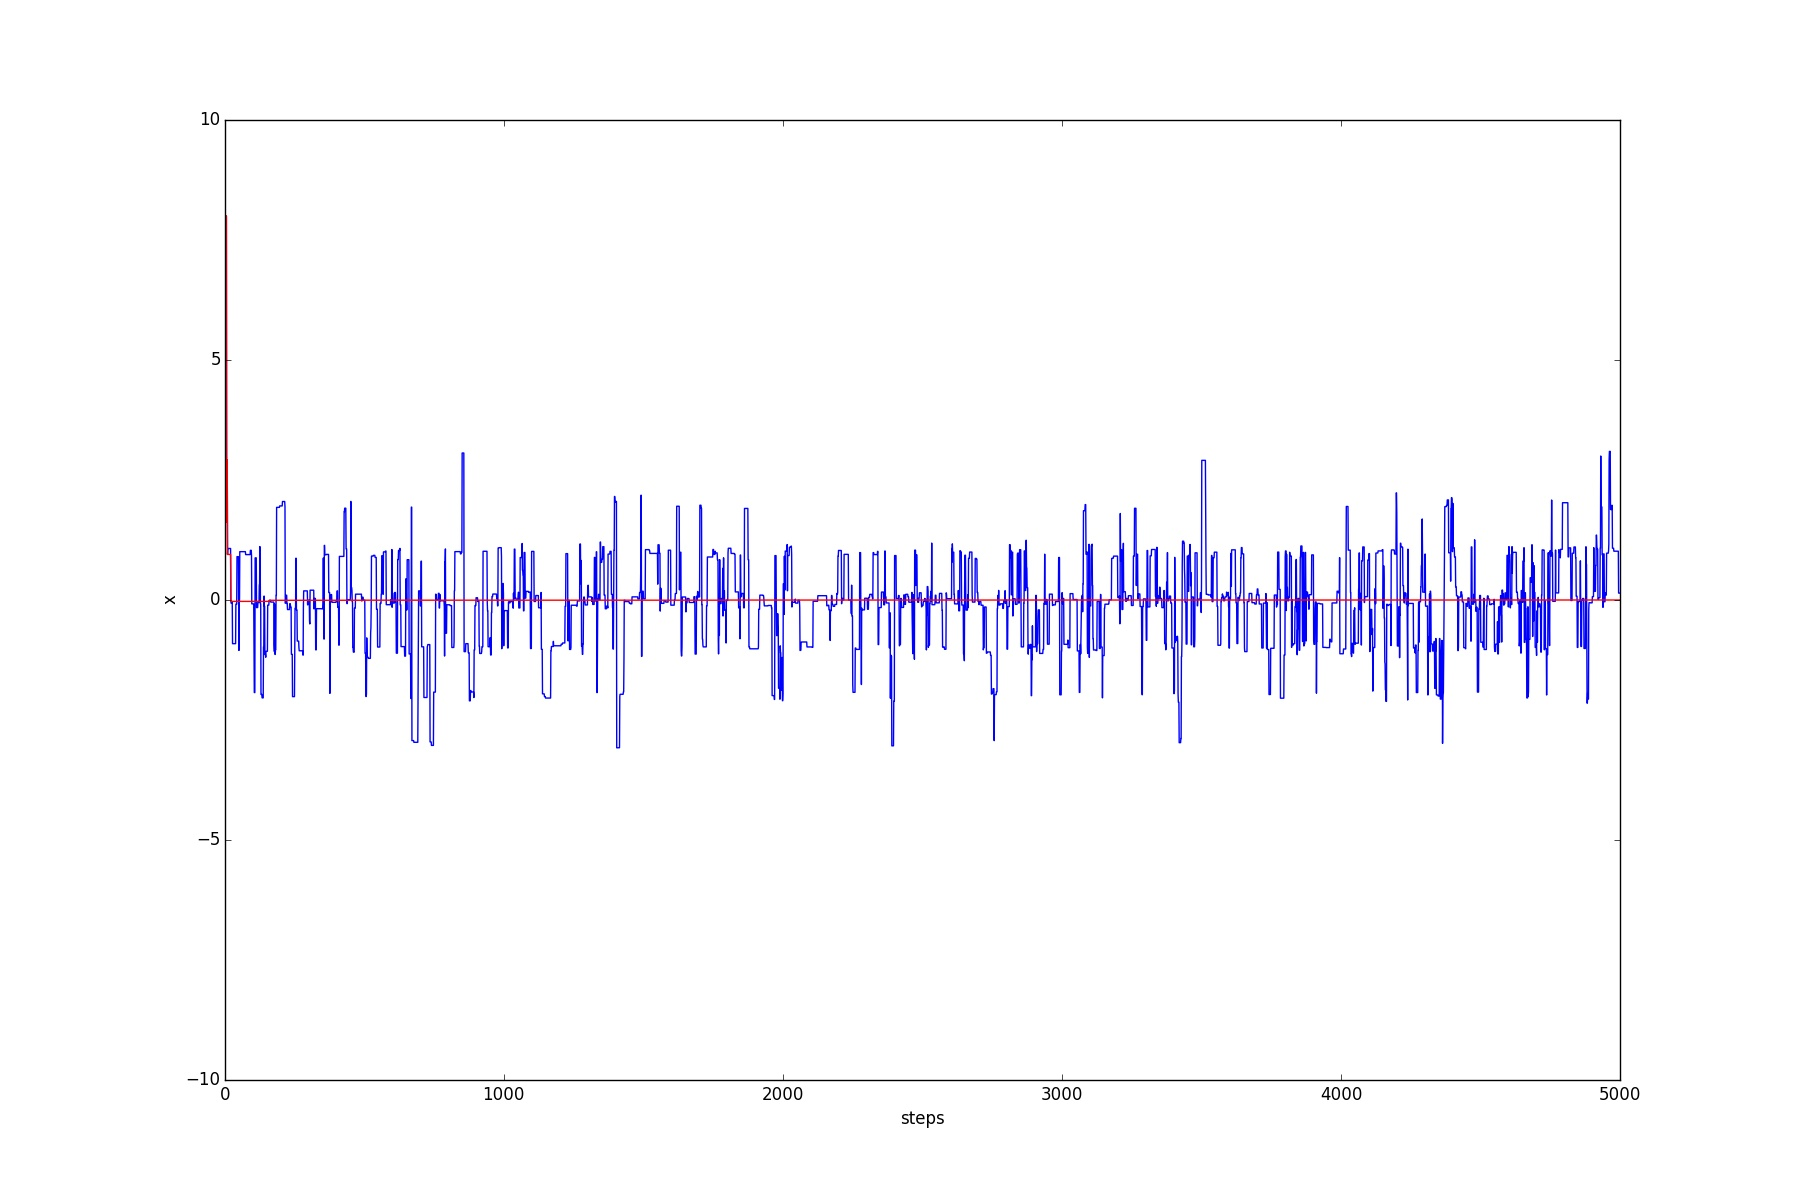
\includegraphics[width=\linewidth]{UQPlot_Ackley_00_Trace.jpg}
\endminipage\hfill
\minipage{0.33\textwidth}
	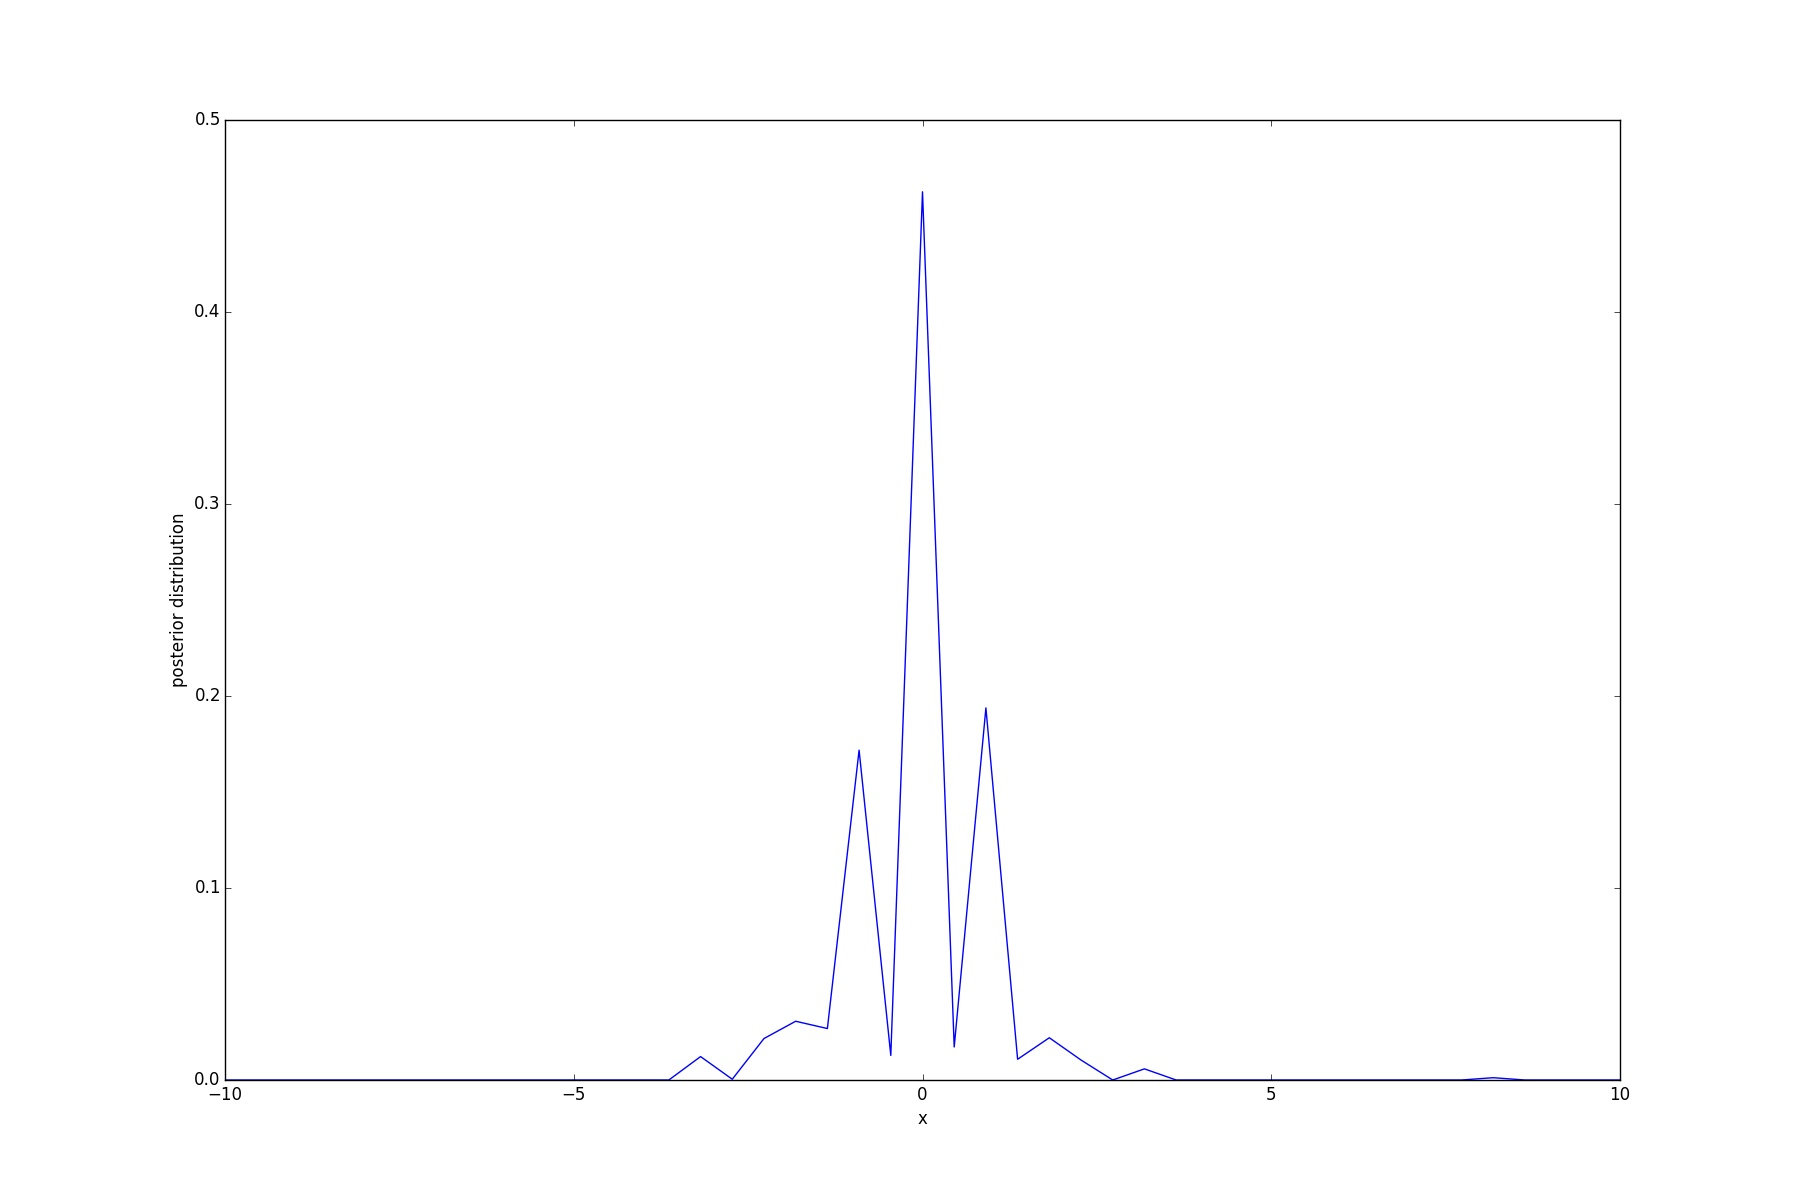
\includegraphics[width=\linewidth]{UQPlot_Ackley_00_Posterior.jpg}
\endminipage
\caption{Plots of the Ackley function (left), chain trace (center), and binned posterior estimate (right) resulting from a run with 5,000 steps. For the posterior plot on the right, we used 50 bins, giving a bin width of 0.4.}
\end{figure}
It is very easy to see from the trace and posterior plots that RSAP efficiently samples the modes near the center.

Lastly, we have a rather illustrative example of the RSAP's performance in the form of a bi-modal function defined by
\begin{equation*}
	f(\theta) = a \Big( 1 - \textrm{exp}(-\dfrac{1}{2} \Big( \dfrac{(\theta-c)^2}{b^2} \Big)^{d/2} ) \Big) + a \Big( 1 - \textrm{exp}(-\dfrac{1}{2} \Big( \dfrac{(\theta+c)^2}{b^2} \Big)^{d/2} ) \Big)
\end{equation*}
where $a = 0.5, b = 0.15, c = 0.333, d = 8, \theta \in [-1, 1]$. The initial state values were set to $\theta^0 = 0.8, \Delta^0 = 0.08$ and the fixed proposal widths were set to $\sigma_\theta = 0.1, \sigma_\Delta = 0.0008$. As discussed above, the parameters for RSAP were set to $\hat A_{t} = 0.1, \hat A_{w} = 10, r_{t} = 0.3, r_{w} = 0.3, n_1 = 2000, n_2 = 1000$.
\begin{figure}[!htb]
\minipage{0.33\textwidth}
	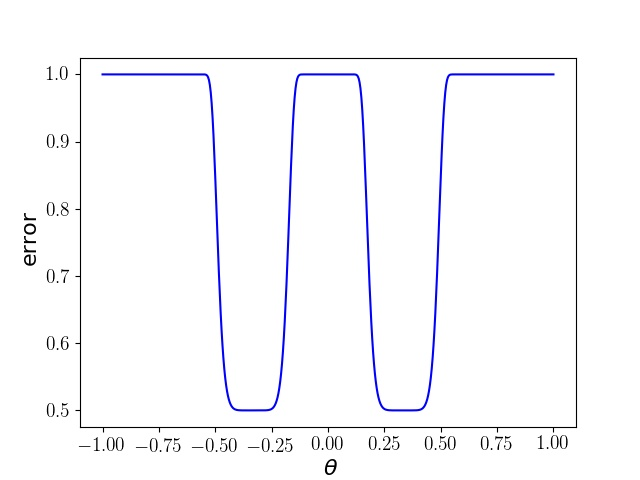
\includegraphics[width=\linewidth]{UQPlot_Bimodal_00_Function.jpg}
\endminipage\hfill
\minipage{0.33\textwidth}
	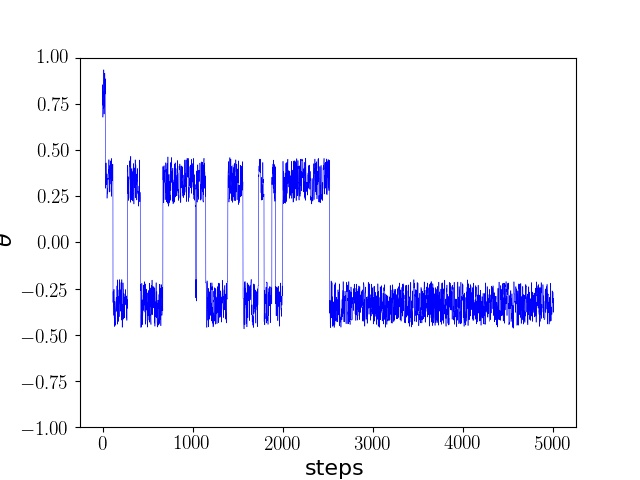
\includegraphics[width=\linewidth]{UQPlot_Bimodal_00_Trace.jpg}
\endminipage\hfill
\minipage{0.33\textwidth}
	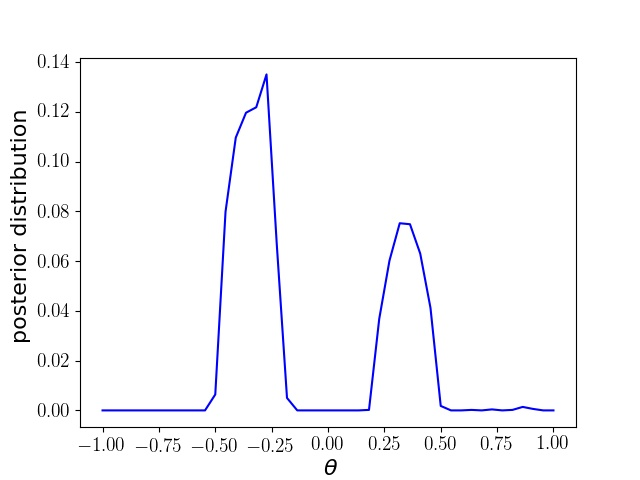
\includegraphics[width=\linewidth]{UQPlot_Bimodal_00_Posterior.jpg}
\endminipage
\caption{Plots of the bi-modal function (left), chain trace (center), and binned posterior estimate (right) resulting from a run with 5,000 steps. For the posterior plot on the right, we used 50 bins, giving a bin width of 0.04.}
\end{figure}
As can be seen, there is efficient mixing between the two modes in the region up until $n = n_1$; however, once standard Metropolis begins to overtake the adaptive effects, the chain becomes temporarily ``stuck" in whichever mode it was currently in. One can simply increase $n_1$ to a suitably large value to maintain the level of mixing efficiency for a longer period of time.

Clearly, these chain mixing tests can be easily skewed by choosing method parameters which work well for RSAP but poor for Metropolis or AM (choosing too small of a proposal width, for example). To alleviate this, the tests in the next section provide a more fair comparison, letting us examine the optimal performance of each method.


\subsection{Convergence to the posterior's global maximum}
We now move on to present results from our optimization-inspired test. This test uses statistics from large ensembles of chains to provide a systematic way of comparing the short-term (i.e., burn-in) performance of Metropolis, Adaptive Metropolis, and RSAP over different proposal widths. This is a valuable test because it shows how quickly on average each method is able to find the global maximum of the posterior for each proposal width. Also, it allows each method to be compared in their optimal context, since sweeping through a large range of proposal widths is guaranteed to contain a near-optimal value. As we shall soon see, RSAP outperforms both Metropolis and Adaptive Metropolis for most proposal widths, particularly in higher dimensionalities.

When performing this test (see Algorithm 3.1), we used $M$-dimensional Ackley functions
\begin{equation*}
	f(\theta) = 20 \bigg( 1 - \textrm{exp}\bigg( -0.2 \Big( \dfrac{1}{M} \sum_{m=1}^{M} \theta_m^2 \Big)^{0.5} \bigg) \bigg) + \bigg( e - \textrm{exp}\bigg( \dfrac{1}{M} \sum_{m=1}^{M} \textrm{cos}(2 \pi \theta_m) \bigg) \bigg)
\end{equation*}
over a domain defined by the $M$-dimensional cube $[-L,L]^M$.
\begin{algorithm}[!t]
\algsetup{
	indent=12pt,
	linenosize=\small,
	linenodelimiter=.
}
\begin{algorithmic}[1]
	\STATE Define the $M$-dimensional parameter vector $\theta^{n}_{i,j}$ as the $n$-th time-step of the $j$-th chain of the $i$-th proposal width
	\FOR{$i = 1$ \TO $N_{width}$}
		\FOR{$j = 1$ \TO $N_{chain}$} % initialize chains
%<<<<<<< HEAD

%			\STATE Initialize chain: $\theta_0^{i,j} \sim U([-L,L]^M)$
%			\STATE Perform Metro/RSAP with initial state $\theta_0^{i,j}$ and fixed proposal covariance matrix $\Sigma^i$
%=======
			\STATE Initialize chain: $\theta^{0,i,j} \sim U([-L,L]^M)$ (note that $\theta^{0,i,j}$ is vector-valued)
			\STATE Calculate the chain $\{ \theta^{0,i,j}, \cdots, \theta^{n,i,j} \}$ for $n = 1, ..., N_{step}$ steps using either Metropolis or RSAP with initial state $\theta^{0,i,j}$ and fixed proposal covariance matrix $\Sigma^i = \sigma^i I$
%>>>>>>> b5fcbc9db7f719088b01834d947fbf38cd06bd54
		\ENDFOR

		\STATE Initialize the cumulative distribution: $c^i_0 = 0$ 
				\FOR{$j = 1$ \TO $N_{chain}$} % check for convergence
			\STATE Initialize convergence check: isConv = false
			\FOR{$n = 1$ \TO $N_{step}$}
				\IF{\NOT isConv \AND $f(\theta^{n,i,j}) \le \epsilon$}
					\STATE $c^i_n = c^i_{n-1} + 1$
					\STATE isConv = true
				\ELSE
					\STATE $c^i_n = c^i_{n-1}$
				\ENDIF
			\ENDFOR
		\ENDFOR
	\ENDFOR
	\STATE Normalize $c$ by dividing all entries by $N_{chain}$
\end{algorithmic}
\caption{Test for convergence to global max}
\end{algorithm}
We sweep through $N_{width}$ proposal widths at equally-spaced intervals, i.e., $\sigma_i = \sigma_{max} (i - 1) / (N_{width}-1)$ where $i = 1, \cdots, N_{width}$.  Obviously, since RSAP adapts the proposal width, we will be sweeping through its \textit{fixed} proposal width, letting these values also equal the widths for Metropolis.  We say ``widths" rather than ``covariance matrices" since---for the Ackley function---each parameter axis is scaled equally, thus causing a single width to work for each. For every width value, we run $N_{chain}$ unique chains (each for $N_{step}$ steps) with initial states that are uniformly-distributed across the hypercubical domain. The cumulative probability of convergence to the global posterior's global maximum versus the time-step is then calculated for each width by determining at which time-step each chain's Ackley evaluation is below the threshold $\epsilon$.

Let us note two more considerations before presenting the results. Since we are merely concerned with the short-term behavior of RSAP, the values $n_1,n_2$ play no role, thus placing us in the adaptive regime the entire time. Also, concerning the value of $\Delta$, lower values are superior for fast initial convergence but not necessarily ideal for accurate sampling of the posterior in the long-term. RSAP, in particular, prefers a low value of $\Delta$, since doing so causes more rejections to occur, letting RSAP adapt more frequently. Thus, we will restrict ourselves to only small values of $\Delta$.

Now, let us examine the results of our numerical tests.
\begin{figure}[t!]%!htb
\minipage{0.333\textwidth}
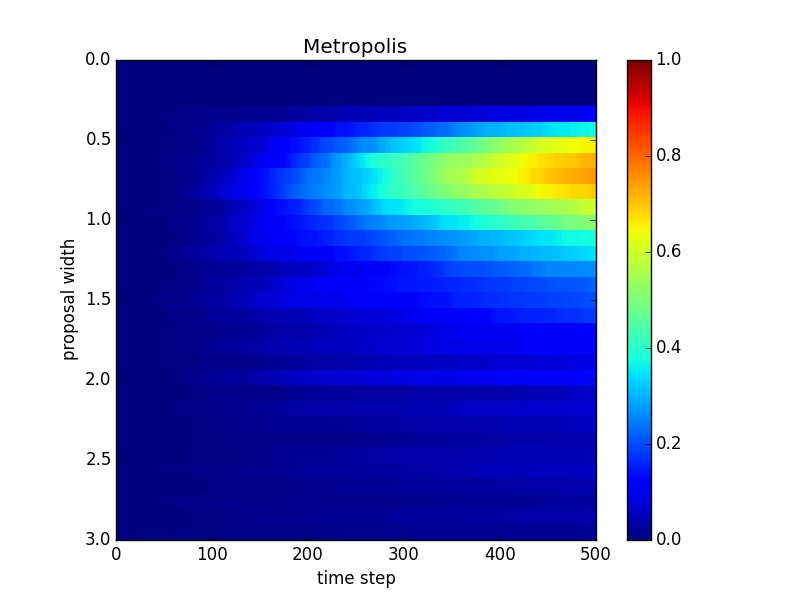
\includegraphics[width=\linewidth]{UQPlot_ConvWidth_Ackley_003D_00_AdaF.jpg}
\endminipage\hfill %%%%%%%%%%%%%%%%%%%
\minipage{0.333\textwidth}
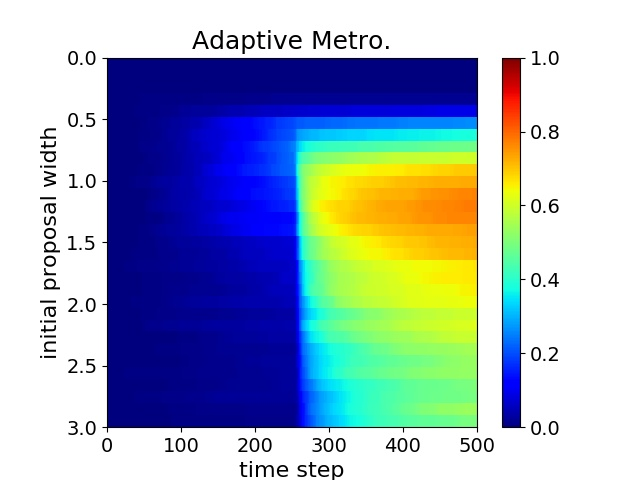
\includegraphics[width=\linewidth]{UQPlot_ConvWidth_Ackley_003D_00_AM.jpg}
\endminipage\hfill %%%%%%%%%%%%%%%%%%%
\minipage{0.333\textwidth}
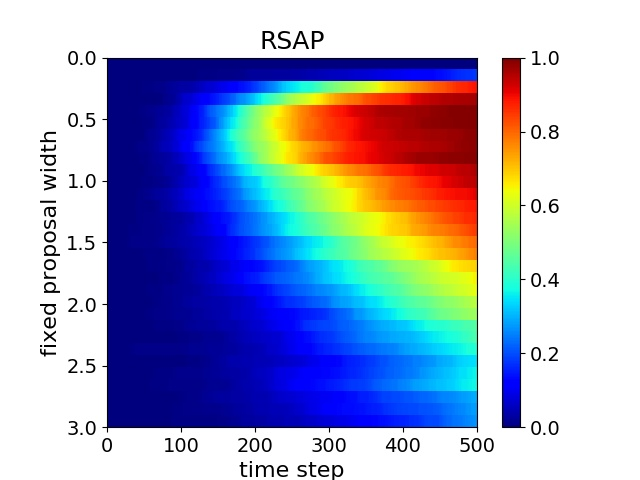
\includegraphics[width=\linewidth]{UQPlot_ConvWidth_Ackley_003D_00_AdaT.jpg}
\endminipage\hfill
\minipage{0.333\textwidth}
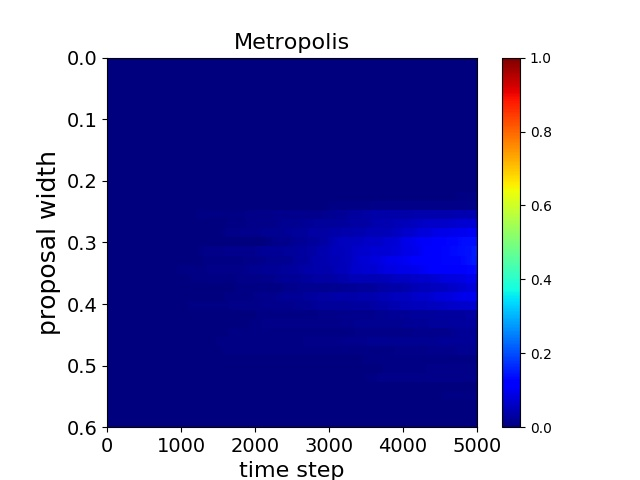
\includegraphics[width=\linewidth]{UQPlot_ConvWidth_Ackley_010D_00_AdaF.jpg}
\endminipage\hfill %%%%%%%%%%%%%%%%%%%
\minipage{0.333\textwidth}
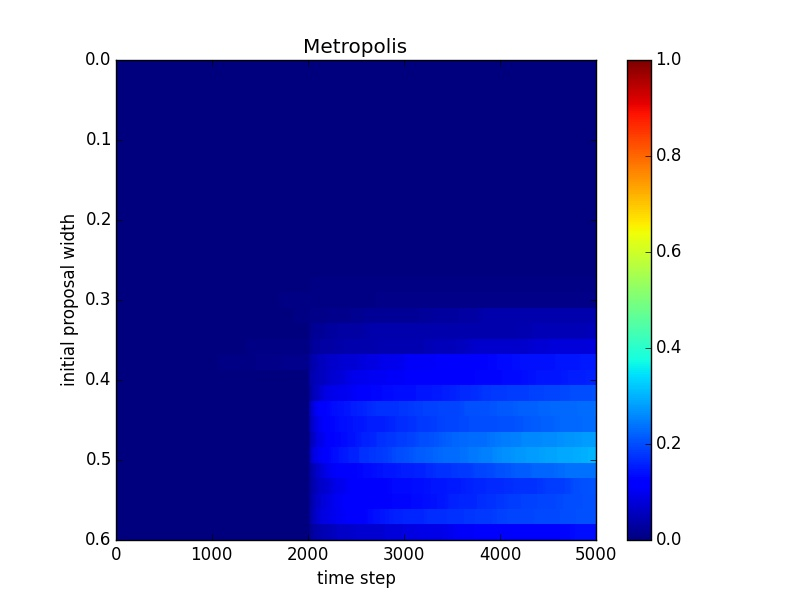
\includegraphics[width=\linewidth]{UQPlot_ConvWidth_Ackley_010D_00_AM.jpg}
\endminipage\hfill %%%%%%%%%%%%%%%%%%%
\minipage{0.333\textwidth}
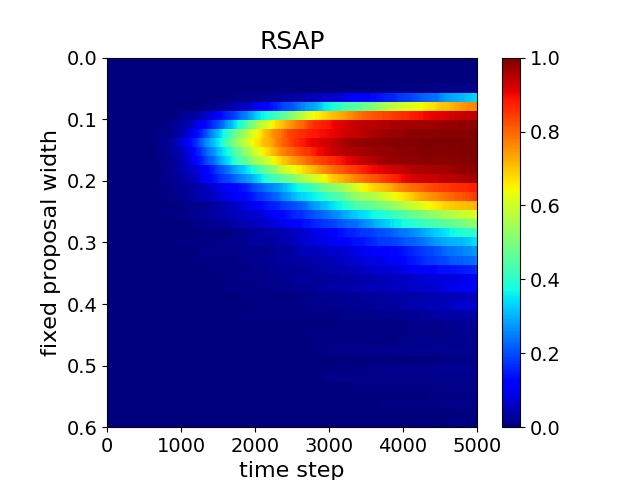
\includegraphics[width=\linewidth]{UQPlot_ConvWidth_Ackley_010D_01_AdaT.jpg}
\endminipage\hfill
\minipage{0.333\textwidth}
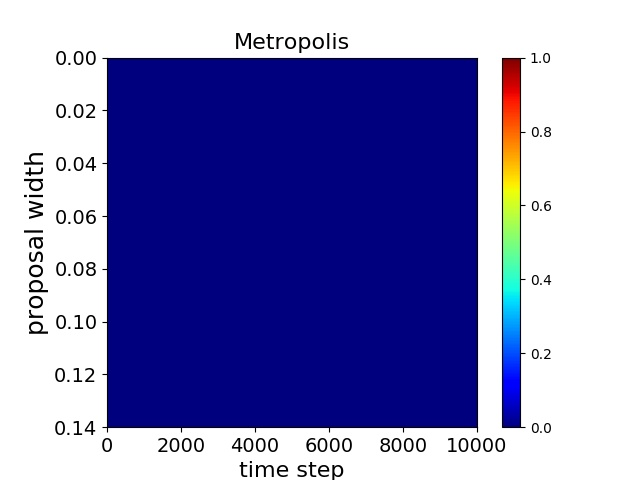
\includegraphics[width=\linewidth]{UQPlot_ConvWidth_Ackley_020D_00_AdaF.jpg}
\endminipage\hfill %%%%%%%%%%%%%%%%%%%
\minipage{0.333\textwidth}
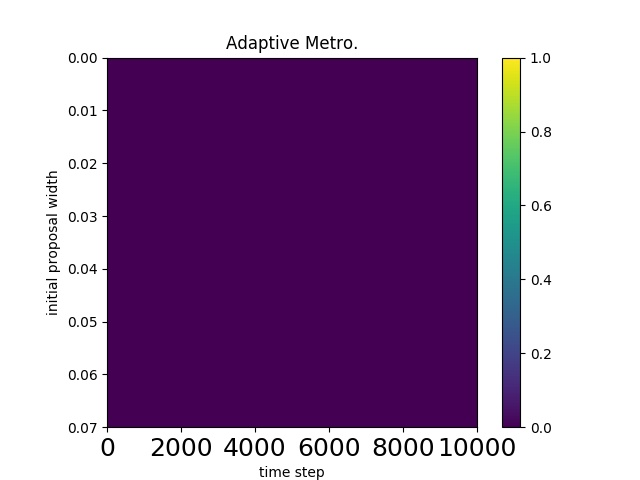
\includegraphics[width=\linewidth]{UQPlot_ConvWidth_Ackley_020D_01_AM.jpg}
\endminipage\hfill %%%%%%%%%%%%%%%%%%%
\minipage{0.333\textwidth}
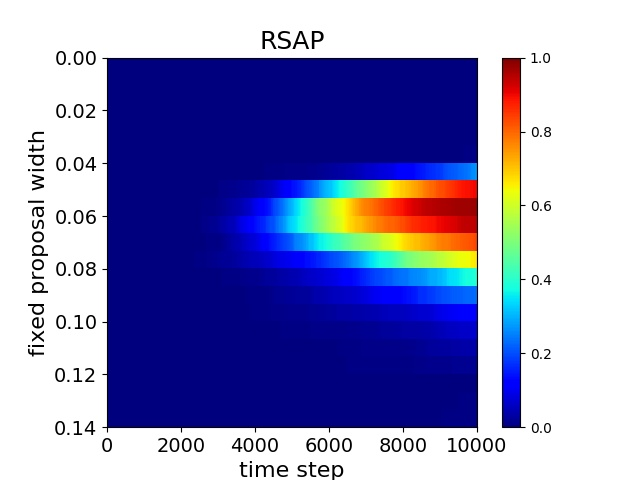
\includegraphics[width=\linewidth]{UQPlot_ConvWidth_Ackley_020D_00_AdaT.jpg}
\endminipage\hfill
\caption{Plots of the cumulative convergence of Metropolis (left), Adaptive Metropolis (center), and RSAP (right) performed on a 3D (top), 10D (center), 20D (bottom) Ackley function. For 3D, we used $N_{burn} = 250$, $\Delta = 0.01$, 5000 time-steps per chain, 500 chains per width value, and threshold of 1.0 over the domain $[-15.0,15.0]^{3}$. For 10D, we used $N_{burn} = 2000$, $\Delta = 0.01$, 5000 time-steps per chain, 500 chains per width value, and threshold of 1.0 over the domain $[-15.0,15.0]^{10}$. For 20D, we used $N_{burn} = 5000$, $\Delta = 0.001$, 10000 time-steps per chain, 500 chains per width value, and threshold of 1.0 over the domain $[-10.0,10.0]^{20}$.}
\label{cumul}
\end{figure}
\begin{table}[t!]
	\centering
	\footnotesize
	\begin{tabular}{ c || c | c | c | c || c | c | c | c || c | c | c | c ||}
		\cline{2-13}
		& \multicolumn{12}{|c|}{Max fraction converged at given run-time completion \%} \\
		\cline{2-13}
%		\hline
		& \multicolumn{4}{|c||}{3D} & \multicolumn{4}{|c||}{10D} & \multicolumn{4}{|c||}{20D} \\
%		\cline{2-13}
		\hline
		\multicolumn{1}{|c||}{run-time \%} & 25\% & 50\% & 75\% & 100\% &    25\% & 50\% & 75\% & 100\% &    25\% & 50\% & 75\% & 100\% \\
		\hline
		\hline
		\multicolumn{1}{|c||}{Metro.} & 0.09 & 0.33 & 0.60 & 0.75 &    0.01 & 0.03 & 0.10 & 0.15 &    0.00 & 0.00 & 0.00 & 0.00 \\
		\hline
		\multicolumn{1}{|c||}{AM} & 0.06 & 0.25 & 0.73 & 0.78 &    0.01 & 0.16 & 0.24 & 0.30 &   0.00 & 0.00 & 0.00 & 0.00 \\
		\hline
		\multicolumn{1}{|c||}{RSAP} & 0.19 & 0.73 & 0.96 & 0.99 &    0.20 & 0.84 & 0.99 & 1.00 &    0.01 & 0.33 & 0.84 & 0.99 \\
		\hline
	\end{tabular}
	\caption{Numeric convergence data from Figure \ref{cumul}. The values are the maximum fraction of converging runs across 4 different time-slices of Figure \ref{cumul} (i.e., the maximum is taken over the range of proposal widths used). The data is grouped by the method used (rows), as well as dimensionality of the problem (columns) and run-time completion percentage (columns). Values were rounded to the nearest hundredth.}
	\label{data}
\end{table}
\begin{comment} % COMMENT!!!!!!!!!
\begin{table}[!htb]
	\centering
	\footnotesize
	\begin{tabular}{ c || c | c | c | c || c | c | c | c || c | c | c | c ||}
		\cline{2-13}
		& \multicolumn{12}{|c|}{Max fraction converged at given run-time completion \%} \\
		\cline{2-13}
%		\hline
		& \multicolumn{4}{|c||}{3D} & \multicolumn{4}{|c||}{10D} & \multicolumn{4}{|c||}{20D} \\
		\cline{2-13}
		& 25\% & 50\% & 75\% & 100\% &    25\% & 50\% & 75\% & 100\% &    25\% & 50\% & 75\% & 100\% \\
		\hline
		\hline
		\multicolumn{1}{|c||}{Metro.} & 0.088 & 0.326 & 0.6 & 0.748 &    0.006 & 0.028 & 0.092 & 0.154 &    0.0 & 0.0 & 0.0 & 0.0\\
		\hline
		\multicolumn{1}{|c||}{AM} & 0.06 & 0.246 & 0.734 & 0.778 &    0.004 & 0.16 & 0.244 & 0.304 &   0.0 & 0.0 & 0.0 & 0.0 \\
		\hline
		\multicolumn{1}{|c||}{RSAP} & 0.188 & 0.726 & 0.96 & 0.996 &    0.2 & 0.844 & 0.99 & 1.0 &    0.004 & 0.334 & 0.836 & 0.976\\
		\hline
	\end{tabular}
	\caption{Numeric convergence data from Figure \ref{cumul}. Values are the maximum fraction of converging runs over all the different proposal widths used.}
	\label{data}
\end{table}
\end{comment}
Figure \ref{cumul} and Table \ref{data} contain the results of a comparison between Metropolis, Adaptive Metropolis, and RSAP on an Ackley function in 3, 10, and 20 dimensions. For the 3D test (top row), there are several features which must be discussed. Observing Figure \ref{cumul}, we notice that both Metropolis and RSAP have relatively similarly shaped convergence profiles, with the fastest rate of convergence happening near some particular optimal value of the proposal width and a tapering off as the width is increased or decreased. The main differences between the two are 1) that RSAP's optimal width is slightly less than that of Metropolis and, more obviously, 2) that RSAP's convergence rate is significantly higher than Metropolis's for all width values. The is confirmed by Table \ref{data}, where we see that RSAP had a near perfect convergence rate within 500 steps while Metropolis only had roughly 75\% convergence. We also notice that many of the RSAP runs converged much earlier in time than those for Metropolis.

On the other hand, the convergence profile for AM is quite different from both Metropolis and RSAP, with its transition into the adaptive regime being very clearly visible at roughly 250 steps. Since AM's proposal width (rather, covariance matrix) should converge to the same value over a large range of initial values, we see similar performance across a wide range of initial widths. Also, though AM's convergence does have an optimal width value, it is much more forgiving than the other two methods when using a suboptimal width. Comparing with Metropolis, Table \ref{data} shows that AM's optimal widths aren't significantly better than standard Metropolis; rather---as previously stated---AM's true benefit lies in its incredibly consistent convergence across a range of different widths. Also, AM outperforms RSAP for larger width values; however, RSAP is still able to outperform both methods when given widths which are smaller than ideal for Metropolis or AM.

Considering just these small width values, it is reasonable for Metropolis and AM to stagnate on the Ackley function if given too small a width. Each trough in the Ackley function has a width of 1.0 between adjacent modes. This is due to the cos$(2 \pi \theta_m)$ term. Now, for a Gaussian distribution, 99.7\% of samples drawn will be within $3 \sigma$ of the mean. Therefore, letting $1.0 = 3 \sigma$, we see that a width of 0.333 will only draw samples outside of a particular trough 0.3\% of the time (assuming that the mean is approximately at the center of the trough, which is reasonable since it will be attracted to that location). If Metropolis were to use such a small width and become trapped in one of Ackley's modes, it would likely take a very large number of steps to escape. Similarly for AM, if its estimation of the optimal width ever became this small, drawing further samples from within the trough would only serve to \textit{decrease} the width estimate even further (AM would have a better chance of escaping such a trough in a low number of dimensions since the coefficient $2.38^2/d > 1$, thus causing the proposal width value to be larger than 0.333). Looking back to the top row of Figure \ref{cumul} (3D), we see no convergence in Metropolis or AM for width values at or below 0.333, with AM actually performing worse than standard Metropolis. On the other hand, due to RSAP's ability to both grow and shrink the width, it still converges well within this region.

% It is also clear how significant the effect of changing the value of $\Delta$ can be, with a value of 0.01 (top row) performing notably superior to 2.0 (bottom row). For both methods, lower $\Delta$ will allow the chains to drift more easily into sub-optimal regions, thus slowing the burn-in process. As stated before, this problem is compounded for RSAP since it depends on rejections to operate effectively.

Moving on, we have a comparison over a 10D Ackley function (center row). Note the scale of the axes has changed dramatically from the 3D case since a 10D space requires more time-steps to explore and the optimal width decreases \cite{SigScale}. In spite of the change of scale, the shape of the three methods' convergence profiles remains similar to their lower-dimensional counterparts, with all three methods having a clear optimal width and AM have more consistent performance across a range of widths, as well as roughly twice the convergence fraction of Metropolis. However, now that we're considering a 10D problem, the superiority of RSAP becomes quite evident, with 100\% convergence of runs within 10000 steps while on Metropolis and AM only achieve 15\% and 30\%, respectively. Also of note is that RSAP's optimal width is now significantly smaller that those of Metropolis or AM.

Finally, we have a comparison over a 20D Ackley function (bottom row). Note again that the axes' scales have changed again). For this test, we shrunk the domain from $[-15.0,15.0]^{20}$ to $[-10.0,10.0]^{20}$ and decreased $\Delta_0$ by a factor of 10. Though it is difficult to tell from the image, we see from the table that there was zero convergence from any of the Metropolis \textit{or} AM runs within 20000 steps. RSAP, on the other hand, still performed quite well, though the range of quickly-converging widths has been greatly compressed. It is clear that the convergence rate of Metropolis and AM in high-dimensional spaces pales in comparison to that of RSAP.

% TABLE:
% average convergecne across a single time slice at 25%, 50%, 75%, 100% of total runtime (for each dimensionality: 3 tables)
% text

\begin{comment}
Use this as impetus for convergence vs. width graphs:

From Haario AP:
"It is well known that when the proposal distribution is too large, too many candidate points are rejected and therefore the chain covers slowly the target distribution. On the other hand, when the proposal distribution is too small, too many candidate points are accepted and the chain converges slowly again. In addition, to ensure computational efficiency one should choose the proposal distribution so that sampling from it would be fast and easy."
\end{comment}


\section{Conclusions}
In this paper, we have presented RSAP---a new adaptive MCMC method---and demonstrated its performance through both analytical and numerical means. Though it performs at an adequately in low-dimensions, its true power lies in its fast convergence in high-dimensional, multimodal spaces, performing better than Metropolis and AM in this particular context.

There are several modifications and applications of RSAP which we would like to investigate in future work. Certainly, different adaptation rules---such as decrementing instead of reseting upon acceptance, scaled incrementing/decrementing based on the acceptance rate, or some type of stochastic incrementing---would be an interesting topic. We also have several ideas on how to combine RSAP and AM in such a way that the resulting method will have the fast convergence of RSAP along with the consistent convergence across a wide range of widths of AM. Lastly, RSAP is an excellent tool for fitting systems of differential equations to some given data. As such, we have an application for RSAP which involves the parameter estimation/best-fit modeling of galaxy mergers. This has been on ongoing project \cite{jspam, citizen} for a number of years now and the application of RSAP will allow us to automate portions of the workflow which currently take a large number of man-hours to complete.

\begin{comment}
Further work:

combine with AM:

1) diagonalizing covariance matrix then applying RSAP

2) let the fixed matrix somehow be the AM matrix (deal with off-diagonals how?)

Alter RSAP by changing adaptation rules and counters:

1) don't reset, just decrement, but add a limit to the counter, maybe increment and decrement at different rates

2) increment and decrement in random floats rather than integers
\end{comment}


%%%%%%%%%%%%%%%
%%%%%%%%%%%%%%%
%%%%% THE END %%%%%
%%%%%%%%%%%%%%%
%%%%%%%%%%%%%%%

\section*{Acknowledgments}
We would like to acknowledge...

\bibliographystyle{siamplain}
\bibliography{references}

\begin{thebibliography}{10}

\bibitem{GelmanBayes} A. Gelman, J ,Carlin, H. Stern, D. Dunson, A. Vehtari, and D. Rubin, \textit{Bayesian Data Analysis}, 3rd ed., CRC Press, 2014.

\bibitem{HaarioAP} H. Haario, E. Saksman, and J. Tamminen, \textit{Adaptive proposal distribution for random walk Metropolis algorithm}, Comput. Stat., 14 (1999), pp. 375-395.

\bibitem{HaarioAM} H. Harrio, E. Saksman, J. Tamminen, \textit{An Adaptive Metropolis Algorithm}, Bernoulli, 7 (2001), pp. 223-242.

\bibitem{Hastings} W. K. Hastings, \textit{Monte Carlo sampling methods using Markov chains and their applications}, Biometrika, 57 (1970), pp. 97-109.

\bibitem{citizen} A. Holincheck, J. Wallin, K. Borne, L. Fortson, C. Lintott, A M. Smith, S. Bamford, W. Keel, and M. Parrish, \textit{Galaxy Zoo: Mergers - Dynamical Models of Interacting Galaxies}, MNRAS, 459 (2016), pp. 720-745.

\bibitem{Interact} L. Jing and P. Vadakkepat, \textit{Interacting MCMC particle filter for tracking maneuvering target}, Digital Signal Processing, 20 (2010), pp. 561-574.

\bibitem{Metro} N. Metropolis, A. W. Rosenbluth, M. N. Rosenbluth, A. H. Teller, and E. Teller, \textit{"Equation of state calculations by fast computing machines}, Journal of Chemical Physics, 21 (1953), pp. 1087-1092.

\bibitem{SigScale} G. O. Roberts, A. Gelman, and W. R. Gilks, \textit{Weak convergence and optimal scaling of random walk Metropolis algorithms}, Ann. Appl. Probab., 7 (1997), pp. 110-120.

\bibitem{AdaptReview} G. O. Roberts and J. S. Rosenthal, \textit{Examples of Adaptive MCMC}, Journal of Computational and Graphical Statistics, 18 (2012), pp. 349-367.%, DOI: 10.1198/jcgs.2009.06134

\bibitem{RRAdaptErgo} G. O. Roberts and J. S. Rosenthal. \textit{Coupling and Ergodicity of Adaptive Markov Chain Monte Carlo Algorithms}, Journal of Applied Probability, 44 (2007), pp. 458-475

\bibitem{AM_RR} G. O. Roberts, and J. S. Rosenthal, \textit{Examples of adaptive MCMC}, Journal of Computational and Graphical Statistics, 18 (2009), pp. 349-367.

\bibitem{RWM} C. Sherlock, P. Fearnhead, G. O. Roberts, \textit{The Random Walk Metropolis: Linking Theory and Practice Through a Case Study}, Statist. Sci., 25 (2010), pp. 172-190.% doi:10.1214/10-STS327. https://projecteuclid.org/euclid.ss/1290175840

\bibitem{jspam} J. Wallin, A. Holincheck, and A. Harvey, \textit{JSPAM: A restricted three-body code for simulating interacting galaxies.}, Astronomy and Computing, 16 (2016), pp. 26-33. 



% \bibitem{galaxyFE} H. Mo, F. Bosch, and S. White, \textit{Galaxy Formation and Evolution}, 2010, Cambridge University Press.



% Harrio adaptive RWM Comput Stat
% https://link.springer.com/article/10.1007/s001800050022

% file:///D:/Graham/Documents/MTSU_HDD/Research/ApCN%20MCMC.pdf
% file:///D:/Graham/Documents/MTSU_HDD/Research/Handbook%20of%20MCMC.pdf
% 
% 


\end{thebibliography}

\end{document}
